%Preamble
	%\XeTeXinputencoding "GB2312"
	\documentclass[UTF8, nocolorlinks]{pkuthss}
	%\documentclass[UTF8]{pkuthss}
	\bibliographystyle{astron}
	\setCJKmainfont[BoldFont={FZHei-B01S}, ItalicFont={FZKai-Z03S}]{FZJPShuSong-Z01S} % FangZhengFonts
	\setCJKfamilyfont{heiti}[BoldFont={FZXiaoBiaoSong-B05S},AutoFakeSlant]{FZXiaoBiaoSong-B05S}
	\setmainfont{CMU Serif Roman}
	%\usepackage{mathptmx}
	%\usepackage{unicode-math}
	%\setmainfont{Times New Roman}
	%\setsansfont{Myriad Pro}
	%\setmonofont[Scale=MatchLowercase]{Consolas}
	% 若需要按照英文文献在前,中文文献在后排序,请设置“sorting = ecnty”;
	% 若需要按照中文文献在前,英文文献在后排序,请设置“sorting = centy”.
	\usepackage[backend = biber, style = caspervector, utf8, sorting = none]{biblatex}
	\usepackage{amssymb}


	% 提供 Verbatim 环境和 \VerbatimInput 命令.
	\usepackage{fancyvrb}

	% 章节标题
	\CTEXsetup[nameformat={\zihao{-2}\bfseries},titleformat={\zihao{-2}\bfseries}]{chapter}
	\CTEXsetup[format={\zihao{-3}\bfseries\centering}]{section}
	\CTEXsetup[format={\zihao{4}\bfseries}]{subsection}
	\CTEXsetup[format={\normalsize\bfseries}]{subsubsection}
	% 使被强调的内容为红色.
	\newcommand{\myemph}[1]{\emph{#1}}
	% pkuthss 文档模版的版本.
	\newcommand{\docversion}{v1.4 rc3}
	% 设定文档的基本信息.
	\pkuthssinfo{
		cthesisname = {本科生毕业论文}, ethesisname = {Undergraduate Thesis},
		ctitle = {对71个Planck冷团块的CO(1-0)成图研究},
		etitle = {CO (1-0) Mapping Study \\of 71 Planck Cold Clumps},
		cauthor = {孟繁一},
		eauthor = {Fanyi Meng},
		studentid = {00946063},
		date = {二\chinese{0}一三年六月},
		school = {元培学院},
		cmajor = {物理学}, emajor = {Physics},
		direction = {天体物理},
		cmentor = {吴月芳\ 教授}, ementor = {Prof.\ Yuefang Wu},
		ckeywords = {恒星形成,分子云,分子谱线},
		ekeywords = {Star Formation,Molecular Cloud,Molecular Spectrum}
	}
	% 导入参考文献数据库(注意不要省略“.bib”).
	\addbibresource{00946063.bib}
	%Following are the substitution of commonly used text in the paper.
	\newcommand{\vdag}{(v)^\dagger}
	\newcommand{\dd}{{\rm d}}
	\newcommand{\umlte}{\frac{M_{LTE}}{M_\odot}}
	\newcommand{\Planck}{\emph{Planck} }
	\newcommand{\coa}{$\rm ^{12}CO$ }
	\newcommand{\cob}{$\rm ^{13}CO$ }
	\newcommand{\coc}{$\rm C^{18}O$ }
	\newcommand{\coaa}{$\rm^{12}CO(1-0)$ }
	\newcommand{\cobb}{$\rm^{13}CO(1-0)$ }
	\newcommand{\cocc}{$\rm C^{18}O(1-0)$ }
	\newcommand{\multi}{$\times$}
	\newcommand{\vlsr}{${\rm V } _{lsr}$}
	\newcommand{\kms}{$\rm km\ s^{-1}$}
	\newcommand{\ta}{$T_{\rm A}$}
	\newcommand{\texc}{$T_{\rm {ex}}$ }
	\newcommand{\taub}{$\tau _{13}$}
	\newcommand{\tauc}{$\tau _{18}$}
	\newcommand{\tcoa}{$T_{12}$}
	\newcommand{\tcob}{$T_{13}$}
	\newcommand{\tcoc}{$T_{18}$}
	\newcommand{\nb}{$N_{13}$\ }
	\newcommand{\nc}{$N_{18}$\ }
	\newcommand{\nhyd}{$N_{\rm H_2}$\ }
	\newcommand{\nnhyd}{$n_{\rm H_2}$\ }
	\newcommand{\pow}[1]{$\times 10^{#1}$}
	\newcommand{\epm}{$\pm$}
	\newcommand{\pcms}{$\rm cm^{-2}$}
	\newcommand{\sigmath}{$\sigma _{Therm}$\ }
	\newcommand{\sigmant}{$\sigma _{NT}$\ }
	\newcommand{\sigmatd}{$\sigma _{3D}$\ }
	\newcommand{\lp}{lognormal}
	\newcommand{\np}{normal{}{}{}}
	%Following is to insert spectra.
	\newcommand{\insertspec}[1]{
	\includegraphics[width=45mm,height=30mm]{img_spec/{#1}.ps}
	}
	%Following are command to insert maps.
	\newcommand{\insertmap}[1]{
	\begin{minipage}[c]{0.3\textwidth}
	\centering
	\includegraphics[width=48mm,height=42mm]{img_maps/{#1}.eps}
	\end{minipage}
	}
	%Following are command not in AASTeX.
	\newcommand{\jj}{{\rm j}}
	\newcommand{\uph}{$\phi$($^{\circ}$)}
	\newcommand{\apjs}{ApJS}
	\newcommand{\apjl}{ApJL}
	\newcommand{\apj}{ApJ}
	\newcommand{\aap}{A\&A}
	\newcommand{\araa}{ARA\&A}
	\newcommand{\mnras}{MNRAS}
	\newcommand{\nat}{Nature}
	\newcommand{\aj}{AJ}
	\newcommand{\arcsec}{$^{\prime\prime}$}
	\newcommand{\arcmin}{$^{\prime}$}
	\newcommand{\arcdeg}{$^{\circ}$}
	%Following are important numbers used in the text.
	\newcommand{\numallsou}{74\ }
	\newcommand{\numsou}{71\ }
	\newcommand{\numsoutmc}{34\ }
	\newcommand{\numsoupmc}{13\ }
	\newcommand{\numsoucmc}{24\ }

	\newcommand{\numclump}{45\ }

	\newcommand{\numcore}{38\ }
	\newcommand{\numcoretmc}{19\ }
	\newcommand{\numcorepmc}{3\ }
	\newcommand{\numcorecmc}{16\ }

	\newcommand{\numduecomp}{5\ }
	\newcommand{\numcocc}{55\ }
	\newcommand{\numcompofcores}{27\ }
	\newcommand{\numdiffusecomp}{42\ }
	\newcommand{\numvelcomp}{76\ }
	%%%%%%%%%%%Packages added by Fanyi Meng%%%%%%%%%%%%%%
	\usepackage{multirow}
	\usepackage{lscape}
	\usepackage{changepage}
	\usepackage{longtable}
	\usepackage{supertabular}
	\usepackage{booktabs}
	\usepackage{float}
	\usepackage[small]{caption}
	\setlength{\captionmargin}{0.5cm}
	%%%%%%%%%%%%%%%%%%%%%%%%%%%%%%%%%%%%%%%%%%%%%%%%%%%%%
\begin{document}
	% 以下为正文之前的部分.
	\frontmatter
	% 自动生成标题页.
	\maketitle

	% 中英文摘要.
\begin{cabstract}

	本文介绍了对 Taurus/Perseus/California 三个分子云复合体中71个 Planck 冷团块气体成分的成图研究. 我们利用中国科学院紫金山天文台青海观测站的13.7 m 毫米波望远镜进行了\coa、\cob 以及 \coc 分子的 $J=1-0$ 转动跃迁谱线观测.全部\numsou 个Planck冷团块都被探测到有\coaa 和\cobb 的辐射,其中55个被探测到有\cocc 的辐射. 通过空间分布和线心速度的验证, 我们证认出 Taurus 分子云复合体(TMC)、Perseus 分子云复合体(PMC)和 California 分子云复合体(CMC)中分别有 \numsoutmc 个、 \numsoucmc 个和 \numsoupmc 个Planck冷团块.在这些冷团块中,共证认出\numcore 个云核(Core), 其中TMC、PMC和CMC分别有\numcoretmc、\numcorepmc 和\numcorecmc 个云核.对于这些云核,我们通过观测数据计算了观测参量:线心速度(\vlsr )、天线温度(\ta )、谱线宽度(FWHM). 通过这些观测参量我们计算出了各个云核的物理参量. 在局部热动平衡(LTE)假设下应用辐射传能方程,我们得到激发温度(\texc )、气体柱密度(\nhyd ).同时我们还计算了云核的热速度弥散(\sigmath )、非热速度弥散(\sigmant )以及三维速度弥散(\sigmatd ).根据对云核成图的椭圆高斯拟合,我们得到了云核的几何尺度($R$),从而计算出气体数密度(\nnhyd )、LTE质量($M_{LTE}$)、Jeans质量($M_{J}$)和virial质量($M_{vir}$).

	根据这些物理参量,我们发现84\%的云核有:\sigmant $>$\sigmath ,而TMC中84\%的云核和CMC中69\%的云核的柱密度概率分布函数(PDF)呈对数正态分布(K-S检验中$p>0.05$),表明在我们的样本中湍动的支配地位.大多数(TMC中的90\%、CMC中的60\%)云核的$M_{vir}$和$M_{J}$大于$M_{LTE}$,表明云核无明显的重力塌缩迹象.通过对比此气体观测结果和 Planck 获得的尘埃连续谱辐射数据,我们发现60\%云核的气体温度低于其尘埃温度.同时,CO分子的丰度在正常范围之内.经过查找成协源,90\%的团块被证实无成协物.根据这些计算与分析,我们发现这些Planck团块还没处于恒星形成前,分子云中的致密核未充分演化的早期形态.本研究揭示了它们的物理状态和动力学性质.
\end{cabstract}

\begin{eabstract}

	A mapping study towards \numsou Planck Cold Clumps was made with \coaa, \cobb and \cocc lines, at the 13.7 m telescope of Purple Mountain Observatory. For all the clumps, \coaa and \cobb emissions were detected, while for \numcocc of them, \cocc emissions were detected.  Of the \numsou Clumps, \numsoutmc are in Taurus Molecular Complex, \numsoucmc in California  Molecular Complex and \numsoupmc are in Perseus Molecular Complex. In the \numvelcomp velocity components, \numcore cores are found in \numcompofcores clumps, \numcoretmc cores are in TMC, \numcorecmc in CMC and \numcorepmc are in PMC.
    We acquired the observational parameters such as $V_{lsr}$, $T_{A}$ and FWHM of lines. Physical parameters including \texc, \nhyd, \sigmath, \sigmant,  \sigmatd were calculated.

    We found that 84\% of the cores have \sigmant larger than \sigmath and 84\% cores in TMC and 69\% cores in CMC have \nhyd lognormal probability distribution function. These suggest the dominance of turbulence in our cores. Most cores (90\% in TMC and 69\% in CMC) are found with $M_{vir}$ and $M_J$ larger than $M_{LTE}$, indicating these cores are neither going to collapse nor gravitationally bound. To compare with the dust properties revealed by Planck ECC catalog, we investigated the coupling of gas and dust components. We found 60\% of the cores are with dust temperature higher than gas temperature. The objects associated with our sources are checked, for 90\% of the core, no associated objects are found within distance of 55\arcsec to their centers. These facts suggest that our samples represent the very early stage of prestellar cores. This research reveals the physical properties and kinematic characteristics of molecular cores which are in their early evolutionary stages.
\end{eabstract}

	% 自动生成目录.
	\tableofcontents
	% 以下为正文.
	\mainmatter

\chapter{引言}

	\section{冷暗云与恒星形成}\label{Sec.ColdDarkCloud}

		暗云(Dark Cloud),也称为分子云(molecular cloud),是主要由$H_2$分子(其质量分数占绝对优势)组成的在光学波段暗的一类星际介质.其在光学波段的消光$A_V>1^{m}$,故被称为“暗”云\supercite{2007ARA&A..45..339B} . 需要指出的是,这种消光并非由其气体成分造成,而是由其中的尘埃颗粒对光学波段的电磁波产生吸收造成的.由于尘埃的这种吸收作用,造成了对外界辐射的良好屏蔽,使得分子云本身能够保持较低的温度(例如典型的致密结构温度在$10-20\rm\ K$\supercite{1983ApJ...265..223B}),这是我们称其为“冷暗云”(Cold Dark Cloud)的原因.

		分子云呈现“层级状”结构\supercite{1994ApJ...423..681V},通常将其分为分子云(Cloud)、团块(Clump)、云核(Core)三个层次\supercite{2007ARA&A..45..339B,2000prpl.conf...97W}:
		\begin{adjustwidth}{0.5cm}{0cm}
		\begin{description}
			\item[分子云:] 质量一般为$10^3-10^4\ M_{\odot}$,尺度为$2-15\rm\ pc$,平均数密度为$50-500\rm\ cm^{-3}$,速度弥散为$2- 5\rm\ km\ s^{-1}$\supercite{2007ARA&A..45..339B}.典型的分子云有Taurus、Perseus以及Orion等.

			\item[团块:] 质量一般为$50-500\ M_{\odot}$,尺度为$0.3-3\rm\ pc$,平均数密度为$10^3-10^4\rm\ cm^{-3}$,速度弥散为$0.3- 3\rm\ km\ s^{-1}$\supercite{2007ARA&A..45..339B}.典型的团块有B213、L1709等\supercite{2007ARA&A..45..339B}.

			\item[云核:] 质量一般为$0.5-5\ M_{\odot}$,尺度为$0.03-0.2\rm\ pc$,平均数密度为$10^4-10^5\rm\ cm^{-3}$,速度弥散为$0.1- 0.3\rm\ km\ s^{-1}$\supercite{2007ARA&A..45..339B}.典型的云核有L1544、L1498以及B68等\supercite{2007ARA&A..45..339B}.
		\end{description}
		\end{adjustwidth}

		分子云是恒星形成的摇篮.此观点由Bart J. Bok于1946年首次提出\supercite{1948HarMo...7...53B},并在之后的半个多世纪被包括红外和毫米波波段在内的观测所证实\supercite{shu1987star,2007ARA&A..45..339B}.虽然前人对分子云核中的恒星形成做过相当多的研究,但由于之前的选源主要在光学或者红外波段,从而选出的源大都是已经有明显的恒星形成活动的区域,使得人们很难对星前核(prestellar core)进行系统的观测,从而不易研究恒星形成的早期状况.基于此,我们亟需一批更长波段(例如毫米-亚毫米波段)系统地选出的源,从而研究恒星(甚至是云核)形成早期阶段的物理状态. 幸运的是,Planck空间望远镜提供了这样的研究样本.

	\section{Planck团块}

		欧洲航天局于2009年5月发射 Planck空间望远镜,其工作波段为:30、44和70 Hz(以上由LFI接收机实现);100、143、217、353、545和857 Hz(以上由HFI接收机实现)\supercite{2011A&A...536A...1P}.Planck 的早期结果系统地提供了丰富的银河系内冷团块样本:C3PO(Cold Core Catalogue of Planck Objects) 星表包含10,873个冷云核\supercite{2011yCat.8088....0P,2011A&A...536A..23P}.在C3PO表中,915个可靠探测($\rm SNR>15$ 且 $T_{\rm ECC}<14\rm\ K$)的源被归入其子表ECC(Planck Early Release Cold Cores Catalogue)\supercite{2011yCat.8088....0P,2011A&A...536A..23P}.

		对于Planck冷团块中尘埃的物理性质,Planck Collaboration进行了的细致研究,从而揭示了C3PO中的冷团块的柱密度$N_ {\rm H_2} \approx 0.1 \rm - \ 1.6 \times 10^{22} \rm\ cm^{-2}$,并且尘埃温度在10 K到15 K之间\supercite{2011A&A...536A..23P}.这些研究利用三个HFI接收机频率(353、545、857 Hz)测得的流量,同时结合IRAS 3000 GHz波段的数据得出相应结果\supercite{2011A&A...536A..23P,2011A&A...536A..22P}.

		除了Planck Collaboration 对于 Planck 冷团块尘埃成分的研究之外, 对其气体成分的单点观测也已经取得成果. 利用中国科学院紫金山天文台青海观测站的13.7 m 毫米波望远镜,Wu et al (2012)完成了对674个ECC源的\coaa 、\cobb  和\cocc  三谱线单点观测,并且得出了其动力学温度($T_k$)、气体柱密度(\nhyd)以及速度弥散($\sigma$)等物理参量\supercite{wu2012gas}.利用同样的设备,Liu et al (2012)等对Orion分子云复合体中的51个Planck 冷团块做了\coaa 、\cobb  和\cocc  三谱线成图观测\supercite{LiuTie}.本文作为同系列的研究,对Taurus、Perseu、California三个分子云复合体中的71个Planck 冷团块同样做了\coaa 、\cobb  和\cocc  三谱线成图观测.

	\section{研究区域}\label{Sec.TPC}

		\subsection{Taurus分子云复合体}

			Taurus分子云复合体(Taurus Molecular Complex,下文简称TMC)是典型的小质量恒星形成区, 同时也是距离我们最近($D\approx 140\rm\ pc$)的巨分子云\supercite{1987ApJ...322..706D}. 因此,在分辨率有限的情况下,TMC是理想的小质量恒星形成研究样本.

			对于TMC,人们已经有大量的分子谱线观测结果.针对TMC和Ophuichus中的90个“微小光学不透明体”(small visual opaques),Myers (1983), Myers and Benson (1983) 进行了\cob 和 \coc 的观测,并且得出其中的云核几何尺度为$0.1-0.3 \ \rm pc$,质量为$4-30\ \rm M_\odot$以及激发温度\texc $\sim$ 10 K\supercite{1983ApJ...264..517M,1983ApJ...266..309M}.在同一系列的成果中,Meyers et al 对云核的亚音速湍动、CO 外向流、形态等也进行了研究\supercite{1983ApJ...270..105M,1988ApJ...324..907M,1991ApJ...376..561M}.

			在TMC中,人们发现了丰富的气体动力学过程和多个演化阶段的特征.分子外向流首次在大质量恒星形成区被发现,但由于距离过远其并不能被很好地被分辨\supercite{1976ApJ...209L.137Z}.而之后在TMC中L1551被证认为有分子外向流,并且红瓣(red-lobe)和蓝瓣(blue-lobe)能够良好地被分辨\supercite{1980ApJ...239L..17S}.截至2003年2月发现的400个分子外向流中,有11\% 在TMC中\supercite{2004A&A...426..503W}.不仅分子外向流,人们在TMC中也发现了丰富的的分子内向流:例如对T Tau 双星系统\supercite{1994ApJ...425L..45V}和L 1544的研究\supercite{1998ApJ...504..900T}.和恒星形成密切相关的盘状结构也在TMC中被证认出来:例如在HL Tau周围发现的盘状结构\supercite{1991ApJ...382L..31S}以及DM Tau\supercite{1995ApJ...453..384S}.综上,TMC包含从class 0到class III 全部恒星形成阶段的源.这些不同演化阶段的源的特征是恒星形成理论,例如Shu et al (1987) 提出的“恒星形成四个阶段”理论\supercite{shu1987star}的观测基础.

		\subsection{Perseus分子云复合体}

			Perseus分子云复合体(Persues Molecular Complex,下文简称PMC)同样是著名的恒星形成区, 其中有中等质量原恒星被证认\supercite{2010A&A...512A..67L}. 一般认为,PMC的情形介于以TMC为代表的小质量恒星形成区和以Orion巨分子云为代表的大质量恒星形成区之间\supercite{2010ApJ...711..655J}.对于PMC,人们亦有大量研究.

			结合亚毫米和中红外资料,在PMC中已有49个深嵌埋(deeply embedded)年轻星体(young stellar objects,下文简称YSO)被证认\supercite{2007ApJ...656..293J}. 而在毫米波段,针对PMC人们也已经进行过多次CO观测\supercite{1979ApJ...233..163S,1999ApJ...525..318P, 2005A&A...440..151H}.

			PMC的距离为235$\pm$18 pc\supercite{2010A&A...512A..67L}.

		\subsection{California分子云复合体}

			有别于TMC和PMC,在2009年之前,California 分子云复合体(California Molecular Complex,下文简称CMC) 并没有获得足够的重视.对于CMC的开创性工作是Lada et al在2009年作出的,其得出了CMC的距离为$450\pm23\rm\ pc$,空间延伸达80 pc,总质量约为 $10^5 M_\odot$\supercite{2009ApJ...703...52L}.CMC有着和Orion巨分子云相似的距离、质量和形态,但是其恒星形成活跃程度对比Orion巨分子云要低得多\supercite{2009ApJ...703...52L,2010A&A...512A..67L}.

			近期,一项对于CMC区域的成图研究给出了含有78个源的星表\supercite{2013ApJ...764..133H}.其中有60个“致密源”在70 $\mu$m的波段上被证认,所用数据来自Herschel的PACS 和 SPIRE设备\supercite{2013ApJ...764..133H}.而另外18个“冷致密源”则是用的Bolocam 1.1 mm 波段的数据\supercite{2013ApJ...764..133H}.

			由于CMC展示出了相对年轻的演化特征,其可以作为研究冷云核早期演化的理想样本.除了上述的研究,我们仍然迫切需要对CMC做更高分辨率的毫米波观测,以更全面而深入地揭示其中冷云核的物理特性.

	\section{研究目标与方法}

		不同于对尘埃的连续谱观测,观测和研究团块和云核的气体谱线可以对其物理性质、动力学特征、稳定性等方面作深入分析.

		我们采用最常用的气体成分探针:CO.本研究选用了其三种同位素分子并观测其最低两个转动能级间的跃迁辐射:\coaa 、\cobb  和\cocc .

		我们通过对TMC、PMC和CMC中的Planck冷团块(特别是团块中的气体云核)的气体成分谱线成图观测,可以得出这些团块和其中的云核的:

		\begin{adjustwidth}{0.5cm}{0cm}
		\begin{enumerate}
			\item 激发温度(\texc )、热速度弥散(\sigmath )、气体柱密度(\nhyd )、数密度(\nnhyd )等物理性质和物质组成.

			\item 本地静止标准速度(\vlsr )、谱线轮廓、非热速度弥散(\sigmant )、三维速度弥散(\sigmatd )等动力学特征.

			\item 云核的几何尺度($R$)、LTE质量($M_{LTE}$)、Jeans质量($M_{J}$)和virial质量($M_{vir}$)等云核特有的参量.这些参量往往和云核的稳定性以及恒星形成密切相关.
		\end{enumerate}
		\end{adjustwidth}
		
		根据这些参量,我们进行了如下分析:

		\begin{adjustwidth}{0.5cm}{0cm}
		\begin{enumerate}
			\item 通过分析谱线轮廓探究其中是否有分子外向流、内流等剧烈的气体运动过程.

			\item 通过比较\sigmath 和\sigmant , 以及检验云核的柱密度概率分布函数(PDF) 来分析热压力、湍动和重力三者在云核中起的作用.

			\item 通过比较云核的 $M_{LTE}$ 、$M_{J}$和$M_{vir}$讨论云核的稳定性.

			\item 通过比较我们得出的气体成分的温度$T_k$和从ECC源表提供的尘埃温度$T_D$揭示这些云核中气体和尘埃的耦合状况.

			\item 通过比较我们得出的CO柱密度和从ECC源表提供的流量等数据计算出的(由尘埃观测导出的)\nhyd, 我们可以得出CO丰度在这些云核中的情况,同时也可以检验我们计算(有气体谱线观测导出的)\nhyd 时采用的CO丰度值是否合理.

			\item 通过查找与我们的云核成协的源,来验证Planck团块和其中的云核是否是星前核(prestellar core).
		\end{enumerate}
		\end{adjustwidth}

		通过这些分析和讨论,我们一方面可以揭示与验证Planck冷团块的物理性质和演化阶段.另一方面,我们可以通过这些样本,系统地总结典型恒星形成区中年轻云核的物理性质、动力学状态、物质组成等基本情况,使得我们了解恒星形成的早期阶段特征.

		值得一提的是,虽然TMC和PMC已经被较多地研究过,人们之前并没有对CMC足够重视,本研究是国际上最早对CMC进行的有针对性的毫米波观测之一,首次揭示了CMC中年轻冷云核的典型性质.

\chapter{观测方法与数据处理}

	\section{观测设备}
		观测设备为中国科学院紫金山天文台青海观测站13.7 m 望远镜.观测时间为2011年1月至5月.观测的谱线为 $J=1 \rightarrow 0 $ 的  \coa, \cob 和 \coc 谱线.观测模式为OTF(On-The-Fly模式).观测时的设备参数如表 \ref{Fig.Observation}.

		\begin{table}[H]
	        \begin{center}
	        \caption{设备参数\label{Fig.Observation}}
	        \setlength{\tabcolsep}{0.1in}
	        \vspace{0.5em}
	        \begin{tabular}{rl}
	        \toprule
	        \hline
	        天线波束宽度              & 56\arcsec$\times$ 55\arcsec (频率为 92.8 GHz时) \\
	        主波束效率                & $\sim$50\%                               \\
	        指向精度                & 好于 4\arcsec                     \\
	        光谱分辨率               & 对于 \coaa: 0.16 \kms                     \\
	                                & 对于 \cobb, \cocc:  0.17 \kms           \\
	        T$^*_A$ 均方根噪声       & 对于 \coaa: 0.2 K                         \\
	                                & 对于 \cobb, \cocc: 0.1 K               \\
	        OTF 扫描速率            & 20 \arcsec $\rm s^{-1}$\\
	        \hline
	        \bottomrule
	        \end{tabular}
	        \end{center}
        \end{table}

    \section{观测源表}
        所有完成观测的源的源名和坐标参见表 \ref{Tab.SourceList} ,有3个源由于参考位置不合适,为了保证数据的可靠性,被排除出后续讨论,其源名之后有“*”为记.我们将在后续研究中重新选取合适的参考位置进行重新观测.

        本研究的选源无任何倾向性,即随机从Wu et al. (2012)的674源中选了在TMC、PMC和CMC范围之内的\supercite{wu2012gas}.

        \topcaption{{观测源表}}\label{Tab.SourceList}
			%%%%%%%%%%%Supertabular Starts!
			\begin{footnotesize}
			\begin{center}
			\setlength{\tabcolsep}{0.04in}
			%%%%%%%%%%%Table head in first page.
			\tablefirsthead{%
			\toprule
			\hline
				源名         &Glon  &Glat&  RA(J2000)      & DEC(J2000)     & RA(B1950)      & DEC(B1950)  &区域&$\dagger$ \\
							 &deg   &deg & (h m s)         & (d m s)        & (h m s)        & (d m s)     &      &          \\
			\hline}
			%%%%%%%%%%%Table tail (except for last page).
			\tabletail{%
			\bottomrule
			\multicolumn{9}{c}{续下页}\\
			%\hline %It looks better without this line.
			}
			%%%%%%%%%%%Table head in following pages.
			\tablehead{%
			%\hline  %It looks better without this line.
			\multicolumn{9}{c}{接上页}\\
			\toprule
				%\hline %Suggest that it is not a new table by removing this top rule.
				源名         &Glon  &Glat&  RA(J2000)      & DEC(J2000)     & RA(B1950)      & DEC(B1950)  &区域&$\dagger$ \\
							 &deg   &deg & (h m s)         & (d m s)        & (h m s)        & (d m s)     &      &          \\
			\hline}
			%%%%%%%%%%%Table tail in last page.
			\tablelasttail{\hline\bottomrule}
			%%%%%%%%%%%Star data.
			\begin{supertabular}{lllcccclr}
			G153.34-08.00 & 153.34715 &   -8.0086632  & 03 48 42.73 & +44 08 46.62 & 03 45 14.92 & +43 59 37.01   & CMC  & N\\
G154.68-15.34 & 154.68748 &  -15.346058   & 03 30 35.18 & +37 31 28.11 & 03 27 21.01 & +37 21 14.40   & PMC  & N\\
G155.52-08.93 & 155.52245 &   -8.9326496  & 03 54 34.60 & +42 03 48.96 & 03 51 09.75 & +41 55 01.08   & CMC  & N\\
G156.53-08.63 & 156.53319 &   -8.6306944  & 03 59 41.99 & +41 38 26.63 & 03 56 17.21 & +41 29 57.92   & CMC  & N\\
G156.90-08.49 & 156.90672 &   -8.4986649  & 04 01 38.87 & +41 29 43.41 & 03 58 14.09 & +41 21 22.06   & CMC  & Y\\
G156.92-09.72 & 156.9287  &   -9.7264977  & 03 57 26.44 & +40 33 29.15 & 03 54 03.85 & +40 24 52.02   & CMC  & N\\
G157.10-08.70 & 157.10448 &   -8.7061596  & 04 01 41.53 & +41 12 37.45 & 03 58 17.25 & +41 04 16.29   & CMC  & Y\\
G157.12-11.56 & 157.12645 &  -11.567412   & 03 51 59.15 & +39 01 55.10 & 03 48 39.82 & +38 52 57.79   & CMC  & N\\
G157.19-08.81 & 157.19237 &   -8.8193874  & 04 01 38.24 & +41 04 05.05 & 03 58 14.22 & +40 55 43.68   & CMC  & N\\
G157.58-08.89 & 157.58788 &   -8.8948917  & 04 02 54.80 & +40 45 04.96 & 03 59 31.18 & +40 36 48.44   & CMC  & Y\\
G157.60-12.17 & 157.60985 &  -12.177292   & 03 51 49.54 & +38 15 38.76 & 03 48 31.47 & +38 06 40.89   & CMC  & N\\
G157.91-08.23 & 157.91747 &   -8.2347422  & 04 06 32.28 & +41 01 15.73 & 04 03 07.73 & +40 53 13.02   & CMC  & Y\\
G158.20-20.28 & 158.20311 &  -20.284357   & 03 29 19.31 & +31 33 54.87 & 03 26 13.37 & +31 23 37.03   & PMC  & Y\\
G158.22-20.14 & 158.22508 &  -20.145231   & 03 29 47.61 & +31 39 49.38 & 03 26 41.50 & +31 29 33.16   & PMC  & Y\\
G158.24-21.80 & 158.24706 &  -21.803167   & 03 25 13.67 & +30 19 30.39 & 03 22 09.71 & +30 08 58.61   & PMC  & Y\\
G158.37-20.72 & 158.37889 &  -20.722431   & 03 28 41.99 & +31 06 59.39 & 03 25 36.68 & +30 56 39.43   & PMC  & Y\\
G158.40-21.86 & 158.40086 &  -21.863445   & 03 25 35.50 & +30 11 29.55 & 03 22 31.67 & +30 00 59.01   & PMC  & Y\\
G159.01-08.46 & 159.0161  &   -8.4609509  & 04 09 55.13 & +40 06 54.78 & 04 06 31.79 & +39 59 05.11   & CMC  & Y\\
G159.03-08.32 & 159.03807 &   -8.3289795  & 04 10 28.53 & +40 11 46.78 & 04 07 04.98 & +40 03 59.25   & CMC  & Y\\
G159.14-08.76 & 159.14793 &   -8.7627697  & 04 09 20.14 & +39 48 21.73 & 04 05 57.40 & +39 40 29.83   & CMC  & Y\\
G159.16-05.58 & 159.16991 &   -5.5854774  & 04 21 08.38 & +42 04 14.47 & 04 17 40.18 & +41 57 08.54   & CMC  & N\\
G159.21-20.12 & 159.21385 &  -20.125366   & 03 33 17.90 & +31 06 48.54 & 03 30 12.10 & +30 56 44.50   & PMC  & Y\\
G159.65-19.68 & 159.65331 &  -19.688967   & 03 36 04.66 & +31 12 02.60 & 03 32 58.46 & +31 02 08.29   & PMC  & Y\\
G159.67-05.71 & 159.67528 &   -5.7166719  & 04 22 32.37 & +41 37 15.79 & 04 19 04.87 & +41 30 15.43   & CMC  & N\\
G159.82-10.48 & 159.82909 &  -10.484298   & 04 05 49.63 & +38 05 19.15 & 04 02 30.19 & +37 57 13.88   & CMC  & N\\
G160.35-06.37 & 160.35643 &   -6.3731093  & 04 22 34.71 & +40 40 40.18 & 04 19 08.95 & +40 33 40.04   & CMC  & N\\
G160.51-16.84 & 160.51024 &  -16.840801   & 03 47 34.31 & +32 53 12.17 & 03 44 24.67 & +32 43 58.95   & PMC  & Y\\
G160.51-17.07 & 160.51024 &  -17.074787   & 03 46 51.18 & +32 42 28.95 & 03 43 41.85 & +32 33 13.12   & PMC  & Y\\
G160.53-09.84 & 160.53221 &   -9.8400545  & 04 10 37.94 & +38 05 04.82 & 04 07 17.99 & +37 57 18.02   & CMC  & Y\\
G160.53-19.72 & 160.53221 &  -19.72859    & 03 38 58.11 & +30 39 04.72 & 03 35 52.31 & +30 29 20.65   & PMC  & N\\
G160.62-16.70 & 160.6201  &  -16.704443   & 03 48 22.46 & +32 55 21.25 & 03 45 12.68 & +32 46 10.96   & PMC  & Y\\
G161.08-21.78 & 161.08153 &  -21.783081   & 03 34 51.38 & +28 43 51.87 & 03 31 48.37 & +28 33 53.36   & PMC  & N\\
G161.21-08.72 & 161.21336 &   -8.725029   & 04 17 02.75 & +38 24 57.50 & 04 13 41.57 & +38 17 35.66   & CMC  & Y\\
G162.24-09.04 & 162.24608 &   -9.0459471  & 04 19 33.27 & +37 28 03.29 & 04 16 13.43 & +37 20 51.37   & CMC  & N\\
G162.46-08.70 & 162.46581 &   -8.7061596  & 04 21 32.60 & +37 33 04.74 & 04 18 12.44 & +37 26 00.67   & CMC  & Y\\
G162.86-05.24 & 162.86131 &   -5.2482533  & 04 35 48.53 & +39 38 08.62 & 04 32 23.40 & +39 32 01.70   & CMC  & N\\
G163.32-08.42 & 163.32274 &   -8.4232397  & 04 25 31.80 & +37 08 19.15 & 04 22 11.95 & +37 01 30.96   & CMC  & Y\\
G164.13-08.85 & 164.13573 &   -8.8571377  & 04 26 43.25 & +36 15 25.18 & 04 23 24.76 & +36 08 41.79   & CMC  & Y\\
G164.57-24.48 & 164.57518 &  -24.480778   & 03 38 12.61 & +24 36 13.41 & 03 35 14.17 & +24 26 26.86   & TMC  & Y\\
G164.75-24.19 & 164.75096 &  -24.194195   & 03 39 34.02 & +24 42 59.94 & 03 36 35.34 & +24 33 18.21   & TMC  & Y\\
G164.81-05.67 & 164.81688 &   -5.6791844  & 04 40 47.51 & +37 53 40.02 & 04 37 25.07 & +37 47 53.55   & TMC  & N\\
G164.92-12.65 & 164.92674 &  -12.654734   & 04 16 04.53 & +33 03 27.18 & 04 12 51.94 & +32 56 01.81   & TMC  & N\\
G166.99-15.34 & 166.99217 &  -15.346058   & 04 13 42.01 & +29 44 26.31 & 04 10 34.35 & +29 36 51.83   & TMC  & N\\
G168.00-15.69 & 168.00291 &  -15.694481   & 04 15 40.46 & +28 48 00.55 & 04 12 33.93 & +28 40 33.81   & TMC  & Y\\
G168.13-16.39 & 168.13475 &  -16.393131   & 04 13 47.56 & +28 13 22.16 & 04 10 41.95 & +28 05 48.10   & TMC  & Y\\
G169.76-16.15 & 169.76073 &  -16.159975   & 04 19 25.47 & +27 15 16.21 & 04 16 20.77 & +27 08 04.27   & TMC  & Y\\
G169.82-19.39 & 169.82664 &  -19.392105   & 04 09 12.03 & +24 58 39.00 & 04 06 10.93 & +24 50 47.28   & TMC  & Y\\
G169.98-18.97 & 169.98045 &  -18.977402   & 04 10 57.74 & +25 09 42.12 & 04 07 56.29 & +25 01 57.19   & TMC  & Y\\
G170.13-16.06 & 170.13426 &  -16.062908   & 04 20 50.61 & +27 03 29.08 & 04 17 46.07 & +26 56 22.76   & TMC  & Y\\
G170.26-16.02 & 170.2661  &  -16.024094   & 04 21 21.47 & +26 59 29.26 & 04 18 16.99 & +26 52 24.97   & TMC  & Y\\
G170.57-07.85 & 170.57372 &   -7.8580132  & 04 50 38.52 & +32 07 05.91 & 04 47 24.92 & +32 02 00.48   & TMC  & N\\
G170.88-10.92 & 170.88133 &  -10.920865   & 04 40 32.71 & +29 55 42.61 & 04 37 22.97 & +29 49 55.56   & TMC  & Y\\
G171.43-17.36 & 171.43065 &  -17.367682   & 04 20 19.19 & +25 15 38.94 & 04 17 17.04 & +25 08 30.63   & TMC  & Y\\
G171.51-10.59*& 171.51854 &  -10.598125   & 04 43 32.45 & +29 39 25.68 & 04 40 22.93 & +29 33 50.96   & TMC  & Y\\
G172.13-16.93 & 172.13377 &  -16.938259   & 04 23 43.24 & +25 03 07.38 & 04 20 41.16 & +24 56 12.56   & TMC  & N\\
G172.83-05.17 & 172.8369  &   -5.1733398  & 05 07 09.50 & +31 59 19.44 & 05 03 55.27 & +31 55 23.51   & TMC  & Y\\
G172.85-14.74 & 172.85887 &  -14.747349   & 04 33 03.17 & +25 58 33.47 & 04 29 59.36 & +25 52 16.07   & TMC  & Y\\
G172.92-16.74 & 172.92479 &  -16.743393   & 04 26 34.88 & +24 36 58.52 & 04 23 33.20 & +24 30 15.13   & TMC  & Y\\
G172.94-05.49 & 172.94676 &   -5.491785   & 05 06 15.78 & +31 42 39.02 & 05 03 02.03 & +31 38 39.30   & TMC  & Y\\
G173.07-17.89 & 173.0786  &  -17.896084   & 04 23 13.65 & +23 44 29.43 & 04 20 13.27 & +23 37 32.71   & TMC  & Y\\
G173.45-05.43 & 173.45213 &   -5.4355769  & 05 07 52.92 & +31 20 25.45 & 05 04 39.67 & +31 16 32.63   & TMC  & N\\
G173.60-17.89 & 173.60594 &  -17.896084   & 04 24 40.82 & +23 21 57.79 & 04 21 40.84 & +23 15 06.86   & TMC  & N\\
G173.91-16.25 & 173.91356 &  -16.25709    & 04 30 55.66 & +24 13 14.78 & 04 27 54.26 & +24 06 48.88   & TMC  & Y\\
G174.06-15.81 & 174.06737 &  -15.810754   & 04 32 50.26 & +24 23 55.66 & 04 29 48.54 & +24 17 37.46   & TMC  & Y\\
G174.39-13.43 & 174.39696 &  -13.439694   & 04 41 46.05 & +25 40 35.79 & 04 38 42.19 & +25 34 53.96   & TMC  & Y\\
G174.70-15.48 & 174.70457 &  -15.481486   & 04 35 40.77 & +24 08 34.46 & 04 32 39.23 & +24 02 27.81   & TMC  & Y\\
G174.81-15.15*& 174.81444 &  -15.152741   & 04 37 05.01 & +24 16 21.02 & 04 34 03.25 & +24 10 20.08   & TMC  & N\\
G175.16-16.74 & 175.166   &  -16.743393   & 04 32 42.66 & +22 59 28.59 & 04 29 42.75 & +22 53 09.94   & TMC  & Y\\
G175.58-16.60*& 175.58348 &  -16.607105   & 04 34 16.84 & +22 46 21.58 & 04 31 17.14 & +22 40 09.30   & TMC  & N\\
G175.97-20.38 & 175.97899 &  -20.38381    & 04 22 57.43 & +20 02 28.95 & 04 20 01.62 & +19 55 31.30   & TMC  & Y\\
G176.46-21.10 & 176.46239 &  -21.101789   & 04 21 54.04 & +19 13 48.81 & 04 18 59.24 & +19 06 46.99   & TMC  & Y\\
G177.60-20.58 & 177.60497 &  -20.582909   & 04 26 29.82 & +18 45 06.57 & 04 23 35.40 & +18 38 23.09   & TMC  & Y\\
G177.89-20.16 & 177.89061 &  -20.165098   & 04 28 34.65 & +18 48 48.70 & 04 25 40.07 & +18 42 13.56   & TMC  & Y\\
G177.97-09.72 & 177.9785  &   -9.7264977  & 05 04 17.30 & +25 11 00.36 & 05 01 13.18 & +25 06 52.61   & TMC  & Y\\
			\end{supertabular}		
			\end{center}
			$\dagger$:表示有(Y)无(N)IRAC/MIPS成协物.
			\end{footnotesize}
			%%%%%%%%%%%Supertabular Ends!

	\section{数据处理}
        为了处理观测数据,我们使用了IRAM提供的GILDAS软件包\supercite{2000ASPC..217..299G}和SMA提供的MIRIAD软件包\supercite{1995ASPC...77..433S}.OTF的数据在处理前被转换为间隔为30\arcsec 的三维数据矩阵(3-D data cube).

        在观测时,成图范围为20\arcmin \multi 20 \arcmin , 但是我们发现, 由于成图范围只是对于9波束接收机阵列中的中心接收机而言的,在图的边缘时信噪比会显著降低.于是我们为了保证数据质量 舍弃了边缘的数据,只保留了14\arcmin \multi 14 \arcmin 的范围.

\chapter{观测结果与参量计算}

	\section{结果综述}

		我们观测的71个源的空间分布如图 \ref{Fig.SpatialDistribution}.

		\begin{figure}[H]
			\centering
			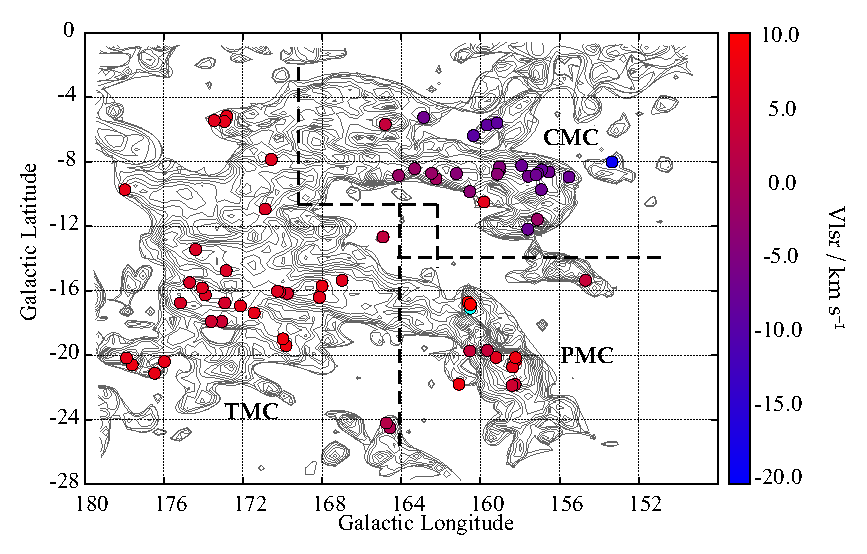
\includegraphics[totalheight=82mm]{img_plot/SpatiaDist_Velocity_Overlay.eps}
			\caption{\small 源的空间分布.背景灰度图来自 1.2 m 望远镜\cob 巡天的积分强度图\supercite{2001ApJ...547..792D},点的颜色代表相应源的几何中心位置的\vlsr .
			虚线表示TMC、PMC、CMC三个区域的分界,根据\parencite{2010A&A...512A..67L}.
			\label{Fig.SpatialDistribution}}
		\end{figure}

		我们在下文以“团块”称这我们观测的源,这是沿用了Planck Collaboration使用的“冷团块”的称呼\supercite{2011A&A...536A..23P}.不仅如此,由于我们的成图区域是14 \arcmin $\times$ 14 \arcmin , 对于TMC、PMC和CMC来说,成图的尺度分别为$0.6\times0.6$ pc、 $0.9\times0.9$ pc、 和 $1.7\times1.7$ pc.这样的成图尺度恰好符合第\ref{Sec.ColdDarkCloud}节中关于团块尺度(0.3$\sim$3 pc)的界定.

		对于\numsou 个团块我们全部探测到了\coaa  和 \cobb 发射线, 而对于其中的 \numcocc 个, 我们探测到了\cocc 发射信号.在5个Planck团块中,我们发现了双重速度成分: 我们检视了每个团块几何中心处的谱线,在这5个源中发现了双重的发射峰;之后为了验证,对于两个峰分别作积分强度图,发现明显分离的辐射区域,从而将其认证为双重速度成分.为了方便和明确,在下文,我们将这10个速度成分视作单独的团块.
	
		我们绘制了全部团块(不同速度成分速度成分视为独立团块)\coaa 和 \cobb 的积分强度图.在本研究中,我们将主要关注云核的性质,是故我们要在团块中证认云核.证认标准为:
		\textbf{在积分强度图中强度为局部峰值的60\% \cob 之等值线需完全包括在成图区域内.}
		这样,我们很好地区分了云核和其所在的团块.同时,由于这样定义的云核有清晰的界限,使得我们可以对其进行较为精确的椭圆高斯拟合.

		为了明确,我们将制定了云核的命名规则:
		\textbf{Planck冷团块名称+a(线心速度小的速度成分)或b(线心速度大的速度成分)或为空(无双重速度成分)+C(云核) + 云核编号 .}

		在所有\numvelcomp 个团块中,\numcompofcores 个含有云核.在这\numcompofcores 个团块其中,我们证认出了总计\numcore 个云核.其中, \numcoretmc 个云核在TMC中、\numcorecmc 个云核在 CMC中,而PMC只有\numcorepmc 个云核.由于PMC中云核过少,我们在后面使用统计方法的分析讨论中将不涉及之.

		在附录\ref{App.Spectra}中,我们出示了每个云核中心位置的光谱;在附录\ref{App.Map}中,我们出示了每个团块的积分强度图.

	\section{观测参量}

		通过对谱线的高斯拟合,我们得到了观测参量:\vlsr、\ta 和 FWHM.每个云核中心处的观测参量如表 \ref{Tab.ObservedPara}.对于全部 \numcore 个云核、 TMC 和 CMC,我们分别对这些观测参量做了统计.统计结果如表 \ref{Tab.ObservedParaStat}.

        我们发现TMC中的云核比之CMC中的云核有着较小的平均$\Delta V (12)$、$\Delta V (13)$ 和 $\Delta V (18)$.但是,TMC中云核的平均$T_{A}(12)$、$T_{A}(13)$ 和 $T_{A}(18)$均比CMC中云核的相应平均值大.



		\begin{landscape}
		\topcaption{{观测参量}}\label{Tab.ObservedPara}
			%%%%%%%%%%%Supertabular Starts!
			\begin{footnotesize}
			\begin{center}
			\setlength{\tabcolsep}{0.04in}
			%%%%%%%%%%%Table head in first page.
			\tablefirsthead{%
			\toprule
			\hline
			云核名称          &  $v_{lsr}$(12)&     FWHM  (12) &   Ta	 (12)           &   $v_{lsr}$(13)   &   FWHM(13)      &  Ta(13)              &     $v_{lsr}$ (18) &  FWHM (18)   &  Ta (18)   &谱线轮廓$^{\dag}$&\\
                   &     (km/s)    &     (km/s)     &     (K)              &         (km/s)    &     (km/s)      &     (K)              &    (km/s)          &     (km/s)   &      (K)   &    &\\
			\hline}
			%%%%%%%%%%%Table tail (except for last page).
			\tabletail{%
			\bottomrule
			\multicolumn{12}{c}{续下页}\\
			%\hline %It looks better without this line.
			}
			%%%%%%%%%%%Table head in following pages.
			\tablehead{%
			%\hline  %It looks better without this line.
			\multicolumn{12}{c}{接上页}\\
			\toprule
			云核名称          &  $v_{lsr}$(12)&     FWHM  (12) &   Ta	 (12)           &   $v_{lsr}$(13)   &   FWHM(13)      &  Ta(13)              &     $v_{lsr}$ (18) &  FWHM (18)   &  Ta (18)   &谱线轮廓$^{\dag}$&\\
                   &     (km/s)    &     (km/s)     &     (K)              &         (km/s)    &     (km/s)      &     (K)              &    (km/s)          &     (km/s)   &      (K)   &    &\\
			\hline}
			%%%%%%%%%%%Table tail in last page.
			\tablelasttail{\hline\bottomrule}
			%%%%%%%%%%%Star data.
			\begin{supertabular}{cccccccccccl}
			G153.34-08.00C1   &-19.14(0.02)   &  2.03(0.04)  &  3.22(0.13)   & -19.06(0.01)   &  1.26(0.03)  &  1.82(0.07)  &  18.98(0.07)  & 1.14(0.17) & 0.27(0.06)&	        &CMC\\
G153.34-08.00C2   &-19.13(0.02)   &  1.57(0.04)  &  3.37(0.18)   & -19.07(0.02)   &  1.05(0.04)  &  1.62( 0.1)  &               &            &           &	        &CMC\\
G154.68-15.34C1   &  3.37(0.07)   &  1.61(0.19)  &  4.09(0.74)   &   3.34(0.01)   &  0.96(0.03)  &  2.59( 0.1)  &               &            &           &	        &PMC\\
G155.52-08.93C1   &	-7.45(0.01)   &  1.08(0.02)  &	3.38(0.06)	 &  -7.45(0.01)	  &  0.80(0.02)	 &  1.57(0.04)  &               &            &           &          &CMC\\											
G156.92-09.72C1   & -7.36(0.02)   &  2.23(0.05)  &  2.54(0.15)   &  -7.24(0.01)   &  1.39(0.03)  &  1.54(0.05)  &  -7.36(0.07)  & 1.12(0.28) & 0.29(0.06)&BA+	      &CMC\\
G157.12-11.56C1   & -1.98(0.02)   &  1.96(0.04)  &  4.44(0.21)   &  -1.68(0.01)   &  1.23(0.02)  &  2.43(0.07)  &  -1.63(0.03)  & 0.87(0.06) & 0.55(0.07)&BA+	      &CMC\\
G157.12-11.56C2   & -1.94(0.02)   &  2.05(0.05)  &   4.3(0.23)   &   -1.7(0.01)   &  1.28(0.03)  &  2.03(0.07)  &  -1.66(0.06)  & 0.88(0.12) & 0.36(0.08)&	        &CMC\\
G157.12-11.56C3   & -1.79(0.02)   &  2.19(0.06)  &  4.58(0.26)   &  -1.72(0.02)   &  1.14(0.05)  &  1.93(0.13)  &               &            &           &	  W     &CMC\\
G157.60-12.17aC1  & -7.61(0.02)   &  2.52(0.05)  &   3.4(0.14)   &  -7.63(0.01)   &  1.43(0.04)  &  2.19(0.42)  &  -7.59(0.04)  & 0.95(0.09) & 0.53(0.07)&	W       &CMC\\
G157.60-12.17bC1  & -2.89(0.01)   &  2.53(0.02)  &  5.44(0.09)   &  -2.57(0.01)   &  1.15(0.03)  &  2.68(0.59)  &   -2.4(0.07)  & 0.71(0.14) & 0.24(0.07)&BA+	      &CMC\\
G157.60-12.17bC2  & -2.44(0.02)   &  2.89(0.04)  &  5.11(0.18)   &  -1.97(0.03)   &  1.82(0.09)  &  1.69(0.11)  &               &            &           &BA+	      &CMC\\
G157.91-08.23C1   & -7.28(0.02)   &  3.25(0.05)  &  2.38(0.11)   &  -7.31(0.01)   &  2.05(0.03)  &  1.92(0.07)  &  -7.49(0.05)  &  1.4( 0.1) & 0.53(0.08)&	        &CMC\\
G159.21-20.12C1   &  6.41(0.01)   &  4.44(0.01)  &  5.75(0.07)   &   6.63(0.01)   &  2.14(0.01)  &  4.88(0.06)  &   6.69(0.01)  &  1.2(0.03) & 1.87(0.06)&RA+	      &PMC\\
G159.67-05.71C1   & -8.72(0.01)   &  2.85(0.03)  &  3.39(0.09)   &  -8.71(0.02)   &  2.01(0.04)  &   1.6(0.08)  &               &            &           &	        &CMC\\
G159.82-10.48C1   &  6.96(0.02)   &  1.87(0.03)  &   4.9( 0.2)   &   7.04(0.02)   &  1.36(0.04)  &  1.91( 0.1)  &               &            &           &BA+,	De  &CMC\\
G160.35-06.37C1   &	-9.34(0.02)   &  1.44(0.05)  &	2.70(0.1)	   &  -9.25(0.02)	  &  1.03(0.04)	 &  1.56(0.05)  &               &            &           &          &CMC\\											
G160.53-19.72C1   &  3.21(0.01)   &  2.33(0.03)  &  5.39(0.15)   &    3.4(0.01)   &  1.85(0.02)  &  2.69(0.07)  &   3.61(0.04)  & 1.17(0.11) & 0.52(0.07)&BA+	      &PMC\\
G162.24-09.04C1   & -0.74(0.02)   &  1.89(0.03)  &   2.5( 0.1)   &   -0.9(0.02)   &  1.48(0.04)  &  1.39(0.08)  &               &            &           &RA+	      &CMC\\
G164.13-08.85C1   & -1.57(0.02)   &  3.27(0.05)  &  2.98(0.12)   &  -1.88(0.02)   &  2.18(0.05)  &  1.26(0.07)  &  -1.87( 0.1)  &  1.4(0.18) & 0.26(0.07)&	        &CMC\\
G164.57-24.48C1   &  0.96(0.01)   &  1.86(0.02)  &  5.09(0.09)   &   0.78(0.01)   &  1.38(0.03)  &  1.49(0.06)  &               &            &           &	  RW    &TMC \\
G164.57-24.48C2   &  1.45(0.01)   &   2.1(0.02)  &  4.92(0.09)   &   1.68(0.01)   &  1.08(0.03)  &   1.5(0.06)  &               &            &           &	  BW    &TMC \\
G164.57-24.48C3   &  1.18(0.01)   &  2.41(0.02)  &  4.88(0.09)   &   0.86(0.02)   &  1.87(0.05)  &  0.95(0.05)  &               &            &           &BA+	      &TMC \\
G164.75-24.19C1   &  1.57(0.01)   &  1.53(0.01)  &  4.19(0.06)   &   1.45(0.01)   &  1.17(0.02)  &  1.29(0.04)  &               &            &           &RA+	      &TMC \\
G164.75-24.19C2   &  1.01(0.01)   &   1.8(0.02)  &  4.67( 0.1)   &   1.09(0.01)   &  1.26(0.03)  &  1.42(0.05)  &               &            &           &	  W     &TMC \\
G164.81-05.67C1   &  3.29(0.01)   &  2.03(0.02)  &  3.12(0.09)   &   3.14(0.02)   &  1.37(0.04)  &  1.91(0.11)  &               &            &           &RA+	      &TMC \\
G164.92-12.65C1   &  2.96(0.03)   &  1.65(0.06)  &  2.44( 0.2)   &   2.87(0.02)   &  0.94(0.05)  &  1.39(0.11)  &               &            &           &BA+	      &TMC \\
G164.92-12.65C2   &  2.95(0.04)   &  2.08(0.08)  &  2.37(0.23)   &   2.86(0.04)   &  1.07(0.09)  &  1.25(0.18)  &               &            &           &	        &TMC \\
G164.92-12.65C3   &  2.98(0.03)   &  2.09(0.06)  &  2.54(0.19)   &   2.83(0.05)   &  1.16(0.11)  &  1.17(0.18)  &               &            &           &	        &TMC \\
G166.99-15.34C1   &  6.61(0.02)   &  3.07(0.04)  &  2.33(0.09)   &   6.62(0.02)   &  1.48(0.04)  &  1.24(0.06)  &   6.76(0.04)  & 0.74( 0.1) & 0.37(0.06)&	  W     &TMC \\
G172.83-05.17C1   &  7.39(0.01)   &  0.91(0.03)  &  3.95( 0.2)   &   7.41(   0)   &  0.58(0.01)  &  2.75(0.06)  &    7.4(0.03)  & 0.39(0.07) & 0.53(0.09)&RA+	      &TMC \\
G172.94-05.49C1   &     7(0.01)   &   0.8(0.01)  &  4.89(0.12)   &   6.98(0.01)   &  0.64(0.01)  &  3.05(0.07)  &   6.98(0.01)  & 0.42(0.02) & 1.06(0.05)&	        &TMC \\
G173.07-17.89C1   &  3.75(0.01)   &  2.03(0.02)  &  4.43( 0.1)   &   3.99(0.01)   &  1.32(0.02)  &  2.39(0.06)  &   4.09(0.04)  & 0.77(0.09) & 0.49(0.06)&	  BW    &TMC \\
G173.07-17.89C2   &  3.61(0.01)   &  2.41(0.02)  &   3.6( 0.1)   &   3.96(0.01)   &  1.33(0.02)  &  2.03(0.06)  &   4.28(0.03)  & 0.34(0.07) & 0.39(0.07)&RA	      &TMC \\
G173.45-05.43C1   &   6.8(0.01)   &  0.62(0.02)  &  4.55(0.16)   &   6.82(0.01)   &  0.48(0.02)  &  2.53(0.09)  &               &            &           &	W       &TMC \\
G173.60-17.89C1   &  4.59(0.01)   &  0.76(0.03)  &  3.44(0.12)   &   4.39(0.01)   &  1.28(0.03)  &  1.78(0.07)  &   4.49(0.07)  &  0.7(0.16) & 0.28(0.07)&BA	      &TMC \\
G173.60-17.89C2   &  3.67(0.02)   &  2.07(0.04)  &  2.77(0.13)   &    3.9(0.01)   &  1.01(0.02)  &  2.07(0.07)  &      4(0.07)  & 0.86(0.21) & 0.23(0.07)&RA+	      &TMC \\
G174.70-15.48C1   &  5.95(   0)   &  2.04(0.02)  &  4.69(0.08)   &   5.87(   0)   &  1.13(0.01)  &  3.65(0.05)  &   5.97(0.01)  & 0.59(0.02) & 1.47(0.05)&	        &TMC \\
G175.97-20.38C1   &  7.17(0.01)   &  1.32(0.03)  &  3.19(0.14)   &   7.26(0.01)   &  1.19(0.03)  &  1.51(0.07)  &               &            &           &RA	      &TMC \\

			\end{supertabular}		
			\end{center}
			\end{footnotesize}
			%%%%%%%%%%%Supertabular Ends!
		\end{landscape}
		
		\begin{table}
			\begin{footnotesize}
	        \begin{center}
	        \caption{观测参量统计结果\label{Tab.ObservedParaStat}}

	        \setlength{\tabcolsep}{0.04in}
	        \vspace{0.5em}

	        \begin{tabular}{lrrrrrrrrr}

\toprule
\hline
&$V_{lsr}$(12)&     $\Delta V$(12)   &   $T_A$(12)    &$V_{lsr}$(13)&     $\Delta V$(13)   &   $T_A$(13)    & $V_{lsr}$(18)&     $\Delta V$(18)   &   $T_A$(18)    \\
&     (km/s)  &     (km/s)     &     (K)              &     (km/s)  &     (km/s)     &     (K)              &      (km/s)  &     (km/s)     &     (K)              \\
\hline
All the \numcore cores &&&&&&&&&\\
\hline
Min.               & -19.14   &0.62   &2.3  &-19.07 &0.48 & 0.95 &-7.59 &0.34  & 0.23\\
Max.               &   7.39   &4.44   &5.8  &  7.41 &2.18 & 4.88 &18.98 &1.40  & 1.87\\
Median             &   1.51   &2.04   &3.8  &  1.56 &1.26 & 1.80 & 4.04 &0.86  & 0.44\\
Mean               &  -0.12   &2.04   &3.8  & -0.08 &1.30 & 1.97 & 2.40 &0.87  & 0.57\\
Standard Deviation &   6.66   &0.75   &1.03 &  6.65 &0.41 & 0.76 & 6.65 &0.32  & 0.45\\
\hline
\numcoretmc cores in TMC &&&&&&&&&\\
\hline
Min.              &   0.96 &  0.62 & 2.33 & 0.78 &0.48  &0.95   & 4.00  &0.34  & 0.23\\
Max.              &   7.39 &  3.07 & 5.09 & 7.41 &1.87  &3.65   & 7.40  &0.86  & 1.47\\
Median            &   3.61 &  2.03 & 3.95 & 3.90 &1.17  &1.51   & 5.23  &0.64  & 0.44\\
Mean              &   3.94 &  1.77 & 3.79 & 3.93 &1.14  &1.86   & 5.50  &0.60  & 0.60\\
Standard Deviation&   2.26 &  0.64 & 0.99 & 2.29 &0.33  &0.72   & 1.43  &0.20  & 0.43\\
\hline
\numcorecmc cores in CMC &&&&&&&&&\\
\hline
Min.              &  -19.14   &  1.08  &  2.38  &  -19.07  &  0.80  &  1.26  &  -7.59  &  0.71 &   0.24 \\
Max.              &    6.96   &  3.27  &  5.44  &    7.04  &  2.18  &  2.68  &  18.98  &  1.40 &   0.55 \\
Median            &   -5.08   &  2.12  &  3.38  &   -4.91  &  1.32  &  1.75  &  -2.13  &  1.03 &   0.33 \\
Mean              &   -5.77   &  2.23  &  3.66  &   -5.69  &  1.42  &  1.82  &  -1.38  &  1.06 &   0.38 \\
Standard Deviation&    6.63   &  0.63  &  0.99  &    6.64  &  0.40  &  0.38  &   8.68  &  0.25 &   0.14 \\
\hline
\bottomrule
\end{tabular}


	        \end{center}
	        \end{footnotesize}
        \end{table}

	\section{物理参量}

		通过已经求得的观测参量我们计算出了各个云核的物理参量. 在局部热动平衡(LTE)假设下应用辐射传能方程,我们可以计算出云核的激发温度(\texc )、气体柱密度(\nhyd )、热速度弥散(\sigmath )、非热速度弥散(\sigmant )以及三维速度弥散(\sigmatd )等物理参量.通过对云核成图进行椭圆高斯拟合,我们还得到了云核的几何尺度($R$),进而计算出气体数密度(\nnhyd )、LTE质量($M_{LTE}$)、Jeans质量($M_{J}$)和virial质量($M_{vir}$).

		我们对于每个云核中各观测位置均计算了物理参量,结合得到的云核边界,我们在云核内部对这些物理参量进行了平均.得到了云核的平均物理参量,如表 \ref{Tab.PhysicalPara}.另外,我们对于全部云核、TMC中的云核以及CMC中的云核分别统计了其平均物理参量的情况,如表 \ref{Tab.PhysicalParaStat}.

		\begin{landscape}
		\topcaption{{物理参量}}\label{Tab.PhysicalPara}
			%%%%%%%%%%%Supertabular Starts!
			\begin{scriptsize}
			\begin{center}
			\setlength{\tabcolsep}{0.08cm}
			%%%%%%%%%%%Table head in first page.
			\tablefirsthead{%
			\toprule
			\hline
			云核名称 & \vlsr& \multicolumn{2}{r}{偏移}  & \multicolumn{3}{r}{几何尺度} & $R$ & \texc& $\tau(^{13}\rm CO)$& \nhyd& \sigmath& \sigmant& \sigmatd& \nnhyd& $M_{LTE}$& $M_{J}$& $M_{vir}$& 区域\\
			&(\kms)&\multicolumn{2}{r}{(\arcsec,\arcsec)} &\multicolumn{3}{r}{(\arcsec$\times$\arcsec(\arcdeg))}&($pc$) &($K$)&&(10$^{21}$ cm$^{-2}$)&(\kms)&(\kms)&(\kms)&(10$^{3}$ cm$^{-3}$) &{($M_{\odot}$)} &{($M_{\odot}$)} &{($M_{\odot}$)}&\\			\hline}
			%%%%%%%%%%%Table tail (except for last page).
			\tabletail{%
			\bottomrule
			\multicolumn{19}{c}{续下页}\\
			%\hline %It looks better without this line.
			}
			%%%%%%%%%%%Table head in following pages.
			\tablehead{%
			%\hline  %It looks better without this line.
			\multicolumn{19}{c}{接上页}\\
			\toprule
			云核名称 & \vlsr& \multicolumn{2}{r}{偏移}  & \multicolumn{3}{r}{几何尺度} & $R$ & \texc& $\tau(^{13}\rm CO)$& \nhyd& \sigmath& \sigmant& \sigmatd& \nnhyd& $M_{LTE}$& $M_{J}$& $M_{vir}$& 区域\\
			&(\kms)&\multicolumn{2}{r}{(\arcsec,\arcsec)} &\multicolumn{3}{r}{(\arcsec$\times$\arcsec(\arcdeg))}&($pc$) &($K$)&&(10$^{21}$ cm$^{-2}$)&(\kms)&(\kms)&(\kms)&(10$^{3}$ cm$^{-3}$) &{($M_{\odot}$)} &{($M_{\odot}$)} &{($M_{\odot}$)}&\\			\hline}
			%%%%%%%%%%%Table tail in last page.
			\tablelasttail{\hline\bottomrule}
			%%%%%%%%%%%Star data.
			\begin{supertabular}{lrrrrrrrrrrrrrrrrrr}
			G153.34-08.00C1 &  -18.93     &        \multicolumn{2}{r}{(6   , -49 ) }       &  \multicolumn{3}{r}{196 $\times$   107  (-13.2)}&      0.158   &  9.7 (0.5)    &  0.82(0.04) &  2.0 (0.7)    &     0.19(0.005)	 &  0.34(0.04)	  & 0.66(0.07)   &  2.0   &   2.9  &  43&19  &CMC\\
G153.34-08.00C2 &  -19.10     &        \multicolumn{2}{r}{(-163, 120 ) }       &  \multicolumn{3}{r}{224 $\times$   86  (-21.0) }&      0.151   &  10.3(0.4)    &  0.65(0.03) &  1.5 (0.4)    &     0.19(0.003)	 &  0.30(0.05)	  & 0.60(0.07)   &  1.6   &   2.0  &  35&17  &CMC\\
G154.68-15.34C1 &  3.31       &        \multicolumn{2}{r}{(216  ,31   ) }      &  \multicolumn{3}{r}{1261$\times$   381   (72.4)}&      0.394   &  11.9(0.9)    &  0.99(0.07) &  2.2 (0.7)    &     0.21(0.008)	 &  0.32(0.09)	  & 0.65(0.14)   &  0.9   &  20    &  76&28  &PMC\\
G155.52-08.93C1 &  -7.46      &        \multicolumn{2}{r}{(18   ,-2   )	}      &  \multicolumn{3}{r}{392 $\times$   284  (-13.8)}&      0.364	&  9.7 (1.0)    &  0.75(0.08) &  1.0 (0.3)    &     0.18(0.009)	 &  0.22(0.05)	  & 0.48(0.07)	 &  0.5	  &   7.8  &  49&15  &CMC\\
G156.92-09.72C1 &  -7.19      &        \multicolumn{2}{r}{(50  , 53  ) }       &  \multicolumn{3}{r}{714 $\times$   421  (-12.7)}&      0.598   &  9.0 (0.4)    &  0.92(0.04) &  1.8 (0.4)    &     0.18(0.004)	 &  0.33(0.08)	  & 0.64(0.13)   &  0.5   &  38    & 160&35  &CMC\\
G157.12-11.56C1 &  -1.79      &        \multicolumn{2}{r}{(-12 , 84  ) }       &  \multicolumn{3}{r}{383 $\times$   238  (-55.4)}&      0.331   &  6.3 (0.9)    &  0.79(0.11) &  3.0 (0.7)    &     0.15(0.010)	 &  0.26(0.05)	  & 0.51(0.08)   &  1.5   &  19    &  53&10  &CMC\\
G157.12-11.56C2 &  -1.90      &        \multicolumn{2}{r}{(-50 , 137 ) }       &  \multicolumn{3}{r}{694 $\times$   269  (-4.7) }&      0.473   &  6.2 (0.7)    &  0.63(0.07) &  2.7 (0.9)    &     0.15(0.009)	 &  0.26(0.06)	  & 0.52(0.09)   &  0.9   &  35    &  77&13  &CMC\\
G157.12-11.56C3 &  -1.62      &        \multicolumn{2}{r}{(-38 , -352) }       &  \multicolumn{3}{r}{173 $\times$   102  (75.9) }&      0.145   &  5.3 (0.2)    &  0.54(0.02) &  2.4 (0.8)    &     0.14(0.003)	 &  0.45(0.08)	  & 0.81(0.13)   &  2.8   &   3.0  &  40&30  &CMC\\
G157.60-12.17C1 &  -7.68      &        \multicolumn{2}{r}{(67  , -45 ) }       &  \multicolumn{3}{r}{405 $\times$   335  (-23.6)}&      0.402   &  10.5(1.0)    &  1.02(0.10) &  2.4 (0.8)    &     0.19(0.009)	 &  0.28(0.09)	  & 0.59(0.13)   &  0.9   &  23    &  76&20  &CMC\\
G157.60-12.17bC1&  -2.55      &        \multicolumn{2}{r}{(-92 , -59 ) }       &  \multicolumn{3}{r}{513 $\times$   372  (39.7) }&      0.476   &  14.9(1.5)    &  0.67(0.07) &  3.0 (0.9)    &     0.23(0.012)	 &  0.21(0.10)	  & 0.54(0.15)   &  1.0   &  40    &  50&14  &CMC\\
G157.60-12.17bC2&  -2.32      &        \multicolumn{2}{r}{(-187, -266) }       &  \multicolumn{3}{r}{281 $\times$   213  (61.4) }&      0.267   &  14.7(1.3)    &  0.40(0.04) &  2.9 (0.9)    &     0.23(0.010)	 &  0.61(0.14)	  & 1.11(0.23)   &  1.8   &  12    & 190&98  &CMC\\
G157.91-08.23C1 &  -7.23      &        \multicolumn{2}{r}{(31  , -106) }       &  \multicolumn{3}{r}{524 $\times$   494  (31.6) }&      0.556   &  8.5 (0.6)    &  1.61(0.11) &  2.8 (0.8)    &     0.17(0.005)	 &  0.41(0.13)	  & 0.77(0.21)   &  0.8   &  51    & 230&47  &CMC\\
G159.21-20.12C1 &  6.53       &        \multicolumn{2}{r}{(47  , 3   ) }       &  \multicolumn{3}{r}{877 $\times$   633  (-32.5)}&      0.425   &  16.1(1.3)    &  1.86(0.15) &  10.7(2.6)    &     0.24(0.010)	 &  0.35(0.13)	  & 0.74(0.21)   &  4.1   & 110    & 130&18  &PMC\\
G159.67-05.71C1 &  -8.50      &        \multicolumn{2}{r}{(-17 , -12 ) }       &  \multicolumn{3}{r}{469 $\times$   418  (-9.4) }&      0.482   &  9.4 (0.6)    &  0.63(0.04) &  2.0 (0.9)    &     0.18(0.006)	 &  0.51(0.13)	  & 0.94(0.20)   &  0.7   &  27    & 410&90  &CMC\\
G159.82-10.48C1 &  7.00       &        \multicolumn{2}{r}{(23  , -7  ) }       &  \multicolumn{3}{r}{453 $\times$   263  (-24.1)}&      0.376   &  12.4(0.7)    &  0.49(0.03) &  2.1 (0.7)    &     0.21(0.006)	 &  0.41(0.09)	  & 0.79(0.14)   &  0.9   &  17    & 150&49  &CMC\\
G160.35-06.37C1 & 	-9.2      &        \multicolumn{2}{r}{(8   , -47 ) }       &  \multicolumn{3}{r}{238 $\times$   79   (43.3)	}&      0.149	&  8.6 (0.7)	&  0.63(0.05) &  1.3 (0.5)    &     0.17(0.008)  &  0.27(0.08) 	  & 0.55(0.11)	 &  1.6	  &   1.7  &  33&12  &CMC\\
G160.53-19.72C1 &  3.56       &        \multicolumn{2}{r}{(6   , 89  ) }       &  \multicolumn{3}{r}{864 $\times$   473  (-62.6)}&      0.364   &  12.8(0.7)    &  0.69(0.04) &  4.2 (1.3)    &     0.21(0.005)	 &  0.34(0.11)	  & 0.71(0.18)   &  1.8   &  33    & 100&23  &PMC\\
G162.24-09.04C1 &  -0.82      &        \multicolumn{2}{r}{(-5  , -19 ) }       &  \multicolumn{3}{r}{562 $\times$   377  (-78.6)}&      0.501   &  8.3 (0.4)    &  0.80(0.04) &  1.6 (0.5)    &     0.17(0.004)	 &  0.37(0.08)	  & 0.70(0.13)   &  0.5   &  23    & 230&45  &CMC\\
G164.13-08.85C1 &  -1.66      &        \multicolumn{2}{r}{(19  , -6  ) }       &  \multicolumn{3}{r}{709 $\times$   372  (35.2) }&      0.559   &  9.9 (0.8)    &  0.54(0.04) &  2.3 (0.7)    &     0.19(0.008)	 &  0.41(0.11)	  & 0.78(0.17)   &  0.7   &  42    & 230&52  &CMC\\
G164.57-24.48C1 &  0.90       &        \multicolumn{2}{r}{(-49 , 90  ) }       &  \multicolumn{3}{r}{226 $\times$   90  (-59.5) }&      0.048   &  12.6(0.6)    &  0.34(0.02) &  1.7 (0.5)    &     0.22(0.005)	 &  0.35(0.07)	  & 0.69(0.11)   &  5.6   &   0.23 &  19&14  &TMC\\
G164.57-24.48C2 &  1.54       &        \multicolumn{2}{r}{(0   , -108) }       &  \multicolumn{3}{r}{285 $\times$   176  (-18.0)}&      0.076   &  12.6(0.6)    &  0.36(0.02) &  1.3 (0.3)    &     0.22(0.005)	 &  0.35(0.08)	  & 0.69(0.13)   &  2.8   &   0.44 &  19&20  &TMC\\
G164.57-24.48C3 &  0.97       &        \multicolumn{2}{r}{(-116, -164) }       &  \multicolumn{3}{r}{190 $\times$   128  (-64.2)}&      0.053   &  12.3(0.8)    &  0.22(0.01) &  1.3 (0.3)    &     0.21(0.006)	 &  0.43(0.09)	  & 0.82(0.13)   &  4.0   &   0.21 &  39&26  &TMC\\
G164.75-24.19C1 &  1.45       &        \multicolumn{2}{r}{(-14 , 98  ) }       &  \multicolumn{3}{r}{145 $\times$   84  (1.6)   }&      0.038   &  11.2(0.7)    &  0.37(0.02) &  1.2 (0.3)    &     0.19(0.006)	 &  0.29(0.04)	  & 0.59(0.06)   &  5.1   &   0.10 &  11& 8.7&TMC\\
G164.75-24.19C2 &  1.07       &        \multicolumn{2}{r}{(-23 , -16 ) }       &  \multicolumn{3}{r}{133 $\times$   81  (-10.8) }&      0.035   &  11.7(1.3)    &  0.36(0.04) &  1.4 (0.5)    &     0.21(0.012)	 &  0.32(0.07)	  & 0.65(0.11)   &  6.6   &   0.10 &  12&10  &TMC\\
G164.81-05.67C1 &  3.10       &        \multicolumn{2}{r}{(30  , 14  ) }       &  \multicolumn{3}{r}{497 $\times$   306  (1.8)  }&      0.132   &  9.3 (1.1)    &  0.94(0.11) &  2.2 (0.6)    &     0.18(0.011)	 &  0.42(0.08)	  & 0.78(0.13)   &  2.8   &   2.2  &  52&27  &TMC\\
G164.92-12.65C1 &  2.85       &        \multicolumn{2}{r}{(-83 , 53  ) }       &  \multicolumn{3}{r}{264 $\times$   104  (-59.7)}&      0.056   &  8.4 (0.9)    &  0.83(0.09) &  1.2 (0.4)    &     0.17(0.010)	 &  0.30(0.06)	  & 0.59(0.09)   &  3.5   &   0.22 &  10&10  &TMC\\
G164.92-12.65C2 &  2.84       &        \multicolumn{2}{r}{(101 , -126) }       &  \multicolumn{3}{r}{342 $\times$   63  (-35.5) }&      0.050   &  8.4 (0.7)    &  0.74(0.06) &  1.2 (0.3)    &     0.17(0.008)	 &  0.36(0.09)	  & 0.68(0.15)   &  4.0   &   0.18 &  12&15  &TMC\\
G164.92-12.65C3 &  2.86       &        \multicolumn{2}{r}{(132 , -167) }       &  \multicolumn{3}{r}{123 $\times$   52  (-44.6) }&      0.027   &  9.4 (0.5)    &  0.61(0.03) &  1.3 (0.3)    &     0.18(0.005)	 &  0.40(0.09)	  & 0.75(0.14)   &  7.6   &   0.055&   7&14.0&TMC\\
G166.99-15.34C1 &  6.49       &        \multicolumn{2}{r}{(-30 , -22 ) }       &  \multicolumn{3}{r}{291 $\times$   199  (-74.3)}&      0.082   &  8.2 (0.3)    &  0.75(0.03) &  1.6 (0.5)    &     0.17(0.003)	 &  0.22(0.09)	  & 0.48(0.15)   &  3.2   &   0.63 &   9& 5.6&TMC\\
G172.83-05.17C1 &  7.45       &        \multicolumn{2}{r}{(-83 , 43  ) }       &  \multicolumn{3}{r}{587 $\times$   410  (19.9) }&      0.167   &  11.5(1.3)    &  1.18(0.13) &  1.5 (0.4)    &     0.20(0.012)	 &  0.11(0.05)	  & 0.41(0.08)   &  1.4   &   2.4  &   5& 5.0&TMC\\
G172.94-05.49C1 &  6.98       &        \multicolumn{2}{r}{(1   , 64  ) }       &  \multicolumn{3}{r}{709 $\times$   482  (14.5) }&      0.198   &  13.1(1.1)    &  0.97(0.08) &  1.9 (0.5)    &     0.22(0.009)	 &  0.12(0.04)	  & 0.44(0.04)   &  1.6   &   4.4  &   7& 5.7&TMC\\
G173.07-17.89C1 &  3.81       &        \multicolumn{2}{r}{(-28 , -19 ) }       &  \multicolumn{3}{r}{609 $\times$   401  (-61.4)}&      0.168   &  11.5(0.6)    &  0.77(0.04) &  2.5 (0.7)    &     0.20(0.005)	 &  0.23(0.07)	  & 0.54(0.12)   &  2.4   &   4.1  &  21& 8.6&TMC\\
G173.07-17.89C2 &  3.89       &        \multicolumn{2}{r}{(120 , -115) }       &  \multicolumn{3}{r}{454 $\times$   283  (24.7) }&      0.122   &  11.1(0.5)    &  0.82(0.04) &  2.4 (0.7)    &     0.20(0.004)	 &  0.10(0.08)	  & 0.37(0.13)   &  3.2   &   2.1  &   3& 2.9&TMC\\
G173.45-05.43C1 &  6.82       &        \multicolumn{2}{r}{(-54 , 72  ) }       &  \multicolumn{3}{r}{531 $\times$   269  (-33.1)}&      0.128   &  12.3(0.7)    &  0.45(0.03) &  1.1 (0.3)    &     0.21(0.005)	 &  0.14(0.02)	  & 0.41(0.02)   &  1.4   &   1.1  &   6& 6.4&TMC\\
G173.60-17.89C1 &  4.17       &        \multicolumn{2}{r}{(101 , -49 ) }       &  \multicolumn{3}{r}{380 $\times$   264  (70.9) }&      0.107   &  9.7 (0.9)    &  0.72(0.07) &  1.8 (0.5)    &     0.19(0.009)	 &  0.21(0.09)	  & 0.47(0.14)   &  2.8   &   1.2  &  11& 6.0&TMC\\
G173.60-17.89C2 &  3.74       &        \multicolumn{2}{r}{(-28 , 113 ) }       &  \multicolumn{3}{r}{273 $\times$   231  (11.1) }&      0.085   &  9.5 (0.7)    &  1.35(0.10) &  1.6 (0.5)    &     0.18(0.006)	 &  0.25(0.07)	  & 0.54(0.12)   &  3.0   &   0.68 &  13& 8.4&TMC\\
G174.70-15.48C1 &  5.86       &        \multicolumn{2}{r}{(-27 , -60 ) }       &  \multicolumn{3}{r}{979 $\times$   651  (65.3) }&      0.271   &  14.0(1.6)    &  1.49(0.17) &  4.0 (1.1)    &     0.22(0.013)	 &  0.17(0.04)	  & 0.50(0.07)   &  2.4   &  17    &  20& 6.9&TMC\\
G175.97-20.38C1 &  7.23       &        \multicolumn{2}{r}{(38  , -32 ) }       &  \multicolumn{3}{r}{148 $\times$   105  (-75.4)}&      0.042   &  9.5 (0.7)    &  0.63(0.05) &  1.1 (0.5)    &     0.18(0.006)	 &  0.32(0.09)	  & 0.63(0.13)   &  4.4   &   0.11 &  12&11.0&TMC\\
			\end{supertabular}		
			\end{center}
			\end{scriptsize}
			%%%%%%%%%%%Supertabular Ends!
		\end{landscape}

		\begin{table}
			\begin{footnotesize}
	        \begin{center}
	        \caption{物理参量统计结果\label{Tab.PhysicalParaStat}}

	        \setlength{\tabcolsep}{0.04in}
	        \vspace{0.5em}

	        \begin{tabular}{lrrrrrrrrrrr}

\toprule
\hline
&$R$ & \texc& $\tau(^{13}\rm CO)$& \nhyd& \sigmath& \sigmant& \sigmatd& \nnhyd& $M_{LTE}$& $M_{J}$& $M_{vir}$\\
&($pc$) &($K$)&&(10$^{21}$ cm$^{-2}$) &(\kms)&(\kms)&(\kms)&(10$^{3}$ cm$^{-3}$) &{($M_{\odot}$)} &{($M_{\odot}$)} &{($M_{\odot}$)}\\
\hline
全部(\numcore) &&&&&&&&&&&\\
\hline
最小值 &0.03  &  5.3  &   0.22  &   1.0  &  0.14  &  0.10  &  0.37  &  0.5 &    0.1 &     3  &    3\\
最小值 &0.60  & 16.1  &   1.86  &  10.7  &  0.24  &  0.61  &  1.11  &  7.6 &  110.0 &   410  &   98\\
中位数 &0.16  & 10.1  &   0.73  &   1.8  &  0.19  &  0.32  &  0.64  &  1.9 &    3.0 &    37  &   14\\
平均值 &0.24  & 10.5  &   0.77  &   2.2  &  0.19  &  0.31  &  0.63  &  2.5 &   14.3 &    70  &   22\\
标准差 &0.18  &  2.4  &   0.36  &   1.6  &  0.02  &  0.11  &  0.16  &  1.8 &   21.7 &    89  &   21\\
\hline
TMC(\numcoretmc) &&&&&&&&&&&\\
\hline
最小值 &0.03  &  8.2  &   0.22  &   1.1  &  0.17  &  0.10  &  0.37  &  1.4  &  0.1  &   3    &   3\\
最小值 &0.27  & 14.0  &   1.49  &   4.0  &  0.22  &  0.43  &  0.82  &  7.6  & 17.0  &  52    &  27\\
中位数 &0.08  & 11.2  &   0.74  &   1.5  &  0.20  &  0.29  &  0.59  &  3.2  &  0.6  &  12    &   9\\
平均值 &0.10  & 10.9  &   0.73  &   1.7  &  0.20  &  0.27  &  0.58  &  3.6  &  2.0  &  15    &  11\\
标准差 &0.07  &  1.8  &   0.35  &   0.7  &  0.02  &  0.11  &  0.13  &  1.7  &  3.9  &  12    &   7\\
\hline
CMC(\numcorecmc) &&&&&&&&&&&\\
\hline
最小值 &0.14  &  5.3  &   0.40  &   1.0  &  0.14  &  0.21  &  0.48  &  0.5  &   1.7 &    33  &   10\\
最小值 &0.60  & 14.9  &   1.61  &   3.0  &  0.23  &  0.61  &  1.11  &  2.8  &  51.0 &   410  &   98\\
中位数 &0.39  &  9.6  &   0.66  &   2.2  &  0.18  &  0.34  &  0.65  &  0.9  &  21.0 &    76  &   25\\
平均值 &0.37  &  9.6  &   0.74  &   2.2  &  0.18  &  0.35  &  0.69  &  1.2  &  21.5 &   128  &   35\\
标准差 &0.16  &  2.7  &   0.28  &   0.6  &  0.03  &  0.11  &  0.17  &  0.7  &  16.1 &   107  &   27\\
\hline
\bottomrule
\end{tabular}


	        \end{center}
	        \end{footnotesize}
        \end{table}

        \subsection{激发温度}

	        在LTE假设下,我们可以认为\texc 在视线方向上为定值,于是可以通过辐射传能方程(radiation transfer equation)得到:

		    \begin{equation}
		    	T_{ex} = T_0 / \ln[T_0 (T^*_R + T_0 \exp{(-T_0/T_{bg})}-1)]
		    \end{equation}

		    $T^*_R$是经过主波束效率改正后的天线温度.$T_0 = h\nu /k$,$k$ 是 Boltzmann 常量. $T_{bg} = 2.73 /k$ 是宇宙微波背景辐射能谱的拟合黑体谱对应的温度.

		\subsection{柱密度}

			在LTE假设下,如果我们假设\cobb 的发射是光薄的,我们可以计算出\cob .采用的方法和Garden et al. (1991)所用方法相同\supercite{1991ApJ...374..540G}.之后我们使用典型的丰度比:$\rm [H_2]/[ ^{12}CO]=10^4$,  $\rm [^{12}CO]/[^{13}CO]=60$来计算\nhyd.(考虑到之前的研究\supercite{1987ApJ...317..926H}证实太阳系附近的$\rm [^{12}CO]/[^{13}CO]\sim 50$而另一研究\supercite{1980Sci...208..663P}揭示$\rm [^{12}CO]/[^{13}CO]\sim 70$:我们采用$\rm [^{12}CO]/[^{13}CO]=60$.)

			由于\numcompofcores 个云核测到有\cocc 的辐射,我们检验了他们的光厚效应:分别用\coc 和\cob 计算其中心附近的\nhyd,并分别记为\nhyd(\coc) 和 \nhyd(\cob).计算方法同前\supercite{1991ApJ...374..540G}.表 \ref{Tab.13/18}显示了对于每个云核用两种同位素计算的\nhyd 数值.图 \ref{Fig.1813}显示了二者的差异.我们发现 ${N_{\rm H_2}(\rm C^{18}O)}/{ N_{\rm H_2}(\rm ^{13}CO)}$ 的范围为从 0.4 到 2.1,平均值为 0.96, 中位数为 0.90, 而其标准差为 0.48.

			\begin{table}
				\begin{center}
				\begin{footnotesize}
				\setlength{\tabcolsep}{0.05cm}
				\caption{由\cob 和 \coc 谱线计算得到的\nhyd 的比较\label{Tab.13/18}}
				\begin{tabular}{lrrrr}
				\toprule
				\hline
				云核名称         &\nhyd(\coc)&\nhyd(\cob)& $\frac{N_{\rm H_2}(\rm C^{18}O)}{N_{\rm H_2}(\rm ^{13}CO)}$  &区域\\
				              &(10$^{21}$ cm$^{-2}$)&(10$^{21}$ cm$^{-2}$)& &\\
				
				\hline
				G153.34-08.00C1  &   2.8	 &  3.1	&0.9   &  CMC \\
				G156.92-09.72C1  &   2.9	 &  2.6	&1.1   &  CMC \\
				G157.12-11.56C1  &   4.0	 &  4.2	&1.0   &  CMC \\
				G157.12-11.56C2  &   2.7	 &  3.6	&0.8   &  CMC \\
				G157.60-12.17C1  &   4.8	 &  3.8	&1.3   &  CMC \\
				G157.60-12.17bC1 &   1.9	 &  5.3	&0.4   &  CMC \\
				G157.91-08.23C1  &   6.6	 &  3.2	&2.1   &  CMC \\
				G159.21-20.12C1  &  27.0     & 10.0	&2.7   &  PMC \\
				G160.53-19.72C1  &   6.4	 &  5.0	&1.3   &  PMC \\
				G164.13-08.85C1  &   3.4	 &  2.1	&1.6   &  CMC \\
				G166.99-15.34C1  &   2.4	 &  2.1	&1.1   &  TMC \\
				G172.83-05.17C1  &   2.1	 &  4.9	&0.4   &  TMC \\
				G172.94-05.49C1  &   4.7	 &  5.7	&0.8   &  TMC \\
				G173.07-17.89C1  &   3.8	 &  4.2	&0.9   &  TMC \\
				G173.07-17.89C2  &   1.3	 &  3.6	&0.4   &  TMC \\
				G173.60-17.89C1  &   1.8	 &  3.0	&0.6   &  TMC \\
				G173.60-17.89C2  &   1.8	 &  3.5	&0.5   &  TMC \\
				G174.70-15.48C1  &   9.6	 &  7.0	&1.4   &  TMC \\
				\hline
				\bottomrule
				\end{tabular}
				\end{footnotesize}
				\end{center}
			\end{table}


			\begin{figure}[H]
				\centering
				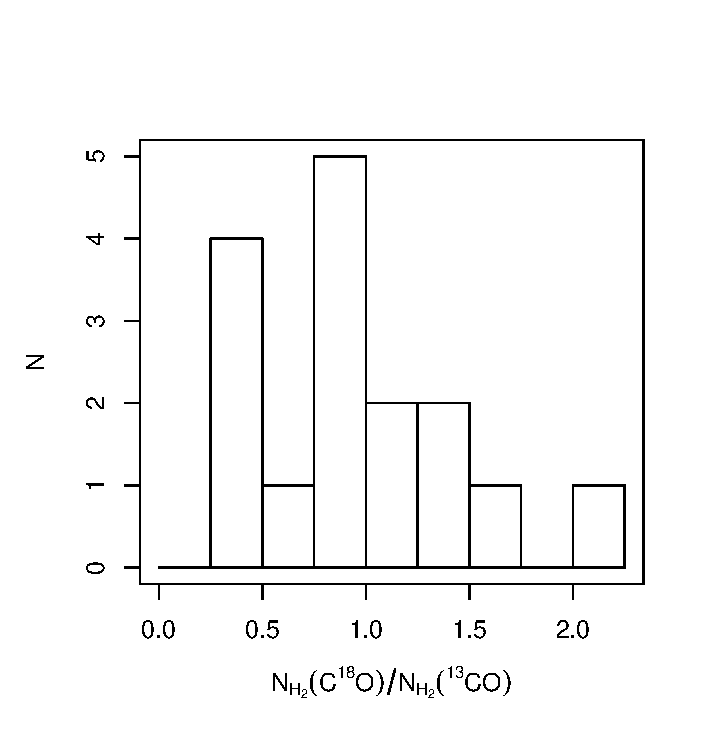
\includegraphics[totalheight=70mm]{img_plot/1813.eps}
				\caption{\small 18个云核的${N_{\rm H_2}(\rm C^{18}O)}/{ N_{\rm H_2}(\rm ^{13}CO)}$分布.}
				\label{Fig.1813}
			\end{figure}

			首先,通过 $\overline{{N_{\rm H_2}(\rm C^{18}O)}/{N_{\rm H_2}(\rm ^{13}CO)}}\approx 1$我们可以看到,在我们的样本中,通过\cob、\coc 两种同位素求得的\nhyd 之间并无系统偏差.这说明光厚效应本身并不显著或我们采用的方法已经考虑了光厚效应并将其很好地反应在了计算结果上,而根据我们的统计,$\tau(^{13}\rm CO)$总体上相对较小,所以至少前者是成立的.

			其次,我们注意到 ${N_{\rm H_2}(\rm C^{18}O)}/{ N_{\rm H_2}(\rm ^{13}CO)}$的统计结果中,标准差高达0.48,这很可能是由我们观测的\cocc 信号的低信噪比造成.

			综合以上两点,同时基于提高精确度的考虑,我们仍然采用\cob 来计算\nhyd.

		\subsection{速度弥散}\label{Sec.VelocityDispersion}

			对于所有的云核,\sigmath 可如下导出:

      		\begin{equation}
      		   \sigma_{Therm}=\left( \frac{kT_{ex}}{m_H \mu} \right)^{1/2}
      		\end{equation}

      		其中,$m_H$ 是H原子的质量, $\mu=2.33 $ 是气体分子的平均质量\supercite{2008A&A...487..993K}(以氢原子质量为单位). 

      		对于无\coc 信号的云核,我们假设\cobb 谱线是光薄的,从而可以计算出\sigmant :

      		\begin{equation}\label{Eq.Calcu_sNT}
      		   \sigma_{NT}=\left(\sigma ^2 _{^{13}{\rm CO}}- \frac{kT_{ex}}{m_{^{13}{\rm CO}}} \right)^{		1/2}
      		\end{equation}

      		其中 $\sigma _{^{13}{\rm CO}} = \frac{\Delta V_{13}}{\sqrt{8\ln2}}$ 是\cob 的一维速度弥散,而$m_{^{13}{\rm CO}}$ 是\cob 的分子质量.

      		而对于有\coc 信号的云核,我们假设\cocc 谱线是光薄的.我们用$\sigma _{\rm C^{18}O}$ 和 $m_{\rm C^{18}O}$ 来替换\ref{Eq.Calcu_sNT}式中的 $\sigma_{^{13}{\rm CO}}$ 和 ${m_{^{13}{\rm CO}}}$,从而可以计算出相应的\sigmant :

      		 \begin{equation}\label{Eq.Calcu_sNT2}
      		   \sigma_{NT}=\left(\sigma ^2 _{{\rm C^{18}O}}- \frac{kT_{ex}}{m_{{\rm C^{18}O}}} \right)^{		1/2}
      		\end{equation}
		
      		结合 \sigmath 与 \sigmant ,我们可以得出 \sigmatd :

      		\begin{equation}
      		   \sigma_{3D}=\sqrt{3(\sigma _{Therm}^2+\sigma _{NT}^2)}
      		\end{equation}

		\subsection{云核参量}

			由于我们证认出的云核具有明确的边界,我们可以估算其几何尺度.而依赖于其尺度的\nnhyd 和 $M_{LTE}$等参量即可求出.为了强调这些参量依赖于我们对云核的证认,特别是依赖于我们对于云核的界定标准,我们统称之为“云核参量”.

			对云核进行椭圆高斯拟合,我们可以得到其椭圆长短轴 $a$、$b$,以及半径$R=\sqrt{ab}D$.其中,$D$是云核的距离,参见第\ref{Sec.TPC}节.

			通过得到的$R$,我们进而可以求出其数密度 $n_{\rm H_2}=N_{\rm H_2} /2R$,由于$R$来自于云核的60\%等值线,我们采用60\%等值线以内的平均\nhyd 而非峰值\nhyd 以避免对\nnhyd 的高估.
			
			最后,我们可以根据上面的云核参量求得$M_{LTE}$(此记号强调这种质量估算是在LTE假设下进行的):
			\begin{equation}
        	 M_{LTE}=\frac{4}{3}\pi R^3 m_H \mu n_{H_2}
      		\end{equation}

      		$m_H$ 是H原子质量,$\mu=2.33$是以$m_H$为单位的平均气体分子质量\supercite{2008A&A...487..993K}.

\chapter{分析与讨论}
	\section{谱线轮廓}

		云核偏离高斯型的谱线轮廓通常是其动力学特征的反映。我们对于本研究中云核发射谱线的非高斯轮廓进行了探究, 对于各谱线形态的界定沿用Wu et al. (2012)单点观测中的判据\supercite{wu2012gas}。

		在TMC的\numcoretmc 个云核中:2个云核的谱线存在蓝色轮廓(blue profile),1个存在蓝不对称(blue asymmetry);4个存在红色轮廓(red profile),2个存在红不对称(red asymmetry)。在PMC仅有的3个云核中,有2个分别被证认分别伴随蓝色、红色轮廓。在CMC的\numcorecmc 个云核的发射谱线中, 有5个发现了蓝色轮廓,1个发现了红色轮廓,2个发现了线翼(wings)。

		各云核的非高斯轮廓形态均列于表 \ref{Tab.ObservedPara}。

		通过P-V图(position-velocity diagram), 我们可以检验谱线存在线翼的云核是否确实具有高速气体(如外向流)\supercite{2005AJ....129..330W}。 

		\begin{figure}[htbp]
		\includegraphics[totalheight=52mm]{img_plot/{pv_G164.75-24.19}.eps}
		\includegraphics[totalheight=52mm]{img_plot/{pv_G173.07-17.89}.eps}
		\caption{云核G164.75-24.19C2和G173.07-17.89C1的P-V图,位置选取参见附录 \ref{Fig.Map}中的图 \ref{Fig.Map}相应积分强度图上的线段标记。\label{Fig.PV}}.
		\end{figure}

		根据P-V图(见图 \ref{Fig.PV})显示,在我们的全部样本中,仅有2个云核展现出高速气体的特征:
		云核G164.75-24.19C2 的P-V图显示了清晰的外向流特征。 而对于云核G173.07-17.89C1,其P-V图上的凸起顶点位置 和云核位置有显著的偏离, 这说明了云核和周围物质有一定的相互作用, 但同时也伴随着高速湍动。

		即便如此,我们的样本中的绝大多数云核并未发现高速气体的存在,这证明了Planck冷团块“年轻”、“安静”的特征,说明我们的选源是成功的。

	\section{云核内的湍动}\label{Sec.Turbulence}

		截至目前的研究揭示:云核尺度的湍动一般是亚音速的,而分子云尺度上湍动是超音速的,相较于热压力,湍动在支撑云核(抵抗重力塌缩)方面作用较小\supercite{1983ApJ...270..105M,2004A&A...416..191T}。然而,对于我们的样本,云核中的湍动较之热运动更加剧烈,占有支配地位。

		我们首先比较了\sigmath 和\sigmant 。如图 \ref{Fig.SigmaTH/SigmaNT},可见在TMC和CMC中大多数云核都有\sigmant / \sigmath $>1$ ,从而其非热运动压力和热压力的比值$R_p=\frac{\sigma^2_{NT}}{\sigma^2_{Therm} }$ 也总体上大于1。而由于只有两个云核中发现了高速气体的迹象,对于大多数云核来说,这种相对而言大的非热速度弥散很可能是湍动占支配地位造成的。

		\begin{figure}[htbp]
		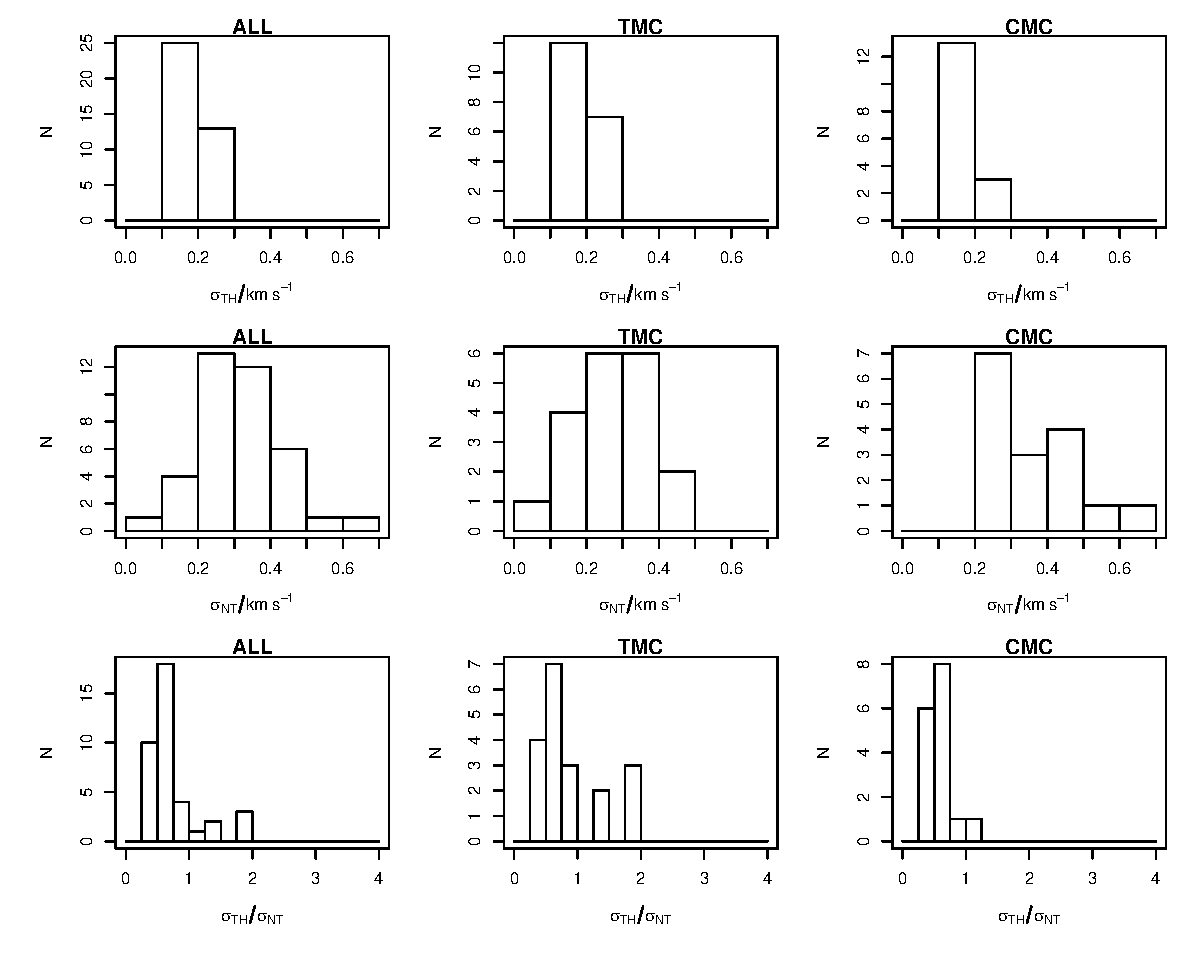
\includegraphics[totalheight=120mm]{img_plot/VelocityComparison.eps}
		\caption{在各个区域中,\sigmath , \sigmant 以及 \sigmath/\sigmant 的分布情况.\label{Fig.SigmaTH/SigmaNT}}
		\end{figure}

		另外,我们还检验了各个云核\nhyd 的概率分布函数(probability distribution function,下文简称为PDF),亦证实此结论。
		理论计算与数值模拟\supercite{2011MNRAS.416.1436B} 以及最近的观测结果\supercite{2013ApJ...766L..17S}均指出:湍动支配下的云核\nhyd 分布会显示出对数正态(lognormal)型的PDF, 而重力因素会使得分布函数在高\nhyd 范围内出现符合幂律分布的情形(power law tail)。 
		为了定量研究我们云核\nhyd 的PDF,我们采用Kolmogorov–Smirnov检验。依惯例,我们设定拒绝空假设的$p$值为0.05。对立假设为\nhyd 符合对数正态(lognormal)分布。

		在TMC的\numcoretmc 个云核中,84\% 展现出对数正态分布的\nhyd PDF;在CMC的\numcorecmc 个云核中,此比例为69\% 。在我们的样本中,未发现高\nhyd 范围内出现幂律分布的迹象。图\ref{Fig.PDF}出示了典型的三个云核(分属于TMC、PMC和CMC)的PDF以及相应的对数正态分布拟合。

		\begin{figure}[htbp]
		\includegraphics[totalheight=62mm]{img_plot/{PDF_G173.60-17.89C2_final}.eps}
		\includegraphics[totalheight=62mm]{img_plot/{PDF_G159.21-20.12C1_final}.eps}
		\includegraphics[totalheight=62mm]{img_plot/{PDF_G157.60-12.17bC2_final}.eps}
		\caption{ TMC、PMC和CMC中典型云核的\nhyd PDF以及相应的对数正态分布拟合\label{Fig.PDF}}.
		\end{figure}

		湍动在这些云核中的支配地位说明我们的样本中罕有重力作用下的塌缩,否则湍动会在一个动力学时标内耗散殆尽\supercite{shu1987star}。这也证实了Planck冷团块的处在演化早期,同时也能说明重力对这些云核的影响并不明显。

	\section{云核的重力稳定性}

		在分子云中,可能有多重作用共同抵抗重力、支持气体成分,例如热压力、湍动、磁场等。考虑到第\ref{Sec.Turbulence}节中我们已经证实了我们的云核中有丰富的湍动,我们将同时考虑热运动和湍动\supercite{2008ApJ...684..395H}来计算$M_{J}$:

     	\begin{equation}
        	\frac{M_{J}}{M_\odot} \approx 1.0a_J \left(\frac{T_{eff}}{10 \rm K}\right)  ^{3/2}  \left(\frac{\mu}{2.33}\right) ^{-1/2} \left(\frac{n^{\rm H_{2}}}{10^4\ \rm cm^{-3}}\right)^{-1/2}
     	\end{equation}

     	其中,$a_J$ 是考虑到维度因素的无量纲量,此处为1. 有效温度 $T_{eff}$ 定义为 :

     	\begin{equation}
         	T_{eff} \equiv \frac{C^2_{s, eff} \mu m_{H}}{k}
     	\end{equation}

     	其中, $C_{s, eff}$ 是等效声速,其定义为:

     	\begin{equation}
       		C_{s, eff} \equiv (\sigma ^2 _{NT}+\sigma ^2 _{Therm})^{1/2}
     	\end{equation}

     	如果我们假定云核是重力束缚的等温球,并且具有骏一的密度且仅仅被随机运动所支撑,其$M_{vir}$可表示为\supercite{2000ApJ...537..221U}:

     	\begin{equation}
        	\frac{M_{vir}}{M_\odot} = 2.10\times 10^{2}\left(\frac{R}{\rm pc}\right)\left(\frac{\Delta V}{\rm km\ s^{-1}}\right)^2
     	\end{equation}

     	其中, $\Delta V $ 是 \coc 或\cob 的FWHM(参见第\ref{Sec.VelocityDispersion}节的讨论)。 由此,我们可以通过比较$M_{vir}$ 和 $M_{LTE}$ 来讨论云核的稳定性。

     	对于TMC和CMC中的云核,我们均进行了$M_{LTE}-M_{J}$以及$M_{LTE}-M_{vir}$的比较,比较结果分别如图 \ref{Fig.Mass}所示。

     	\begin{figure}[htbp]
			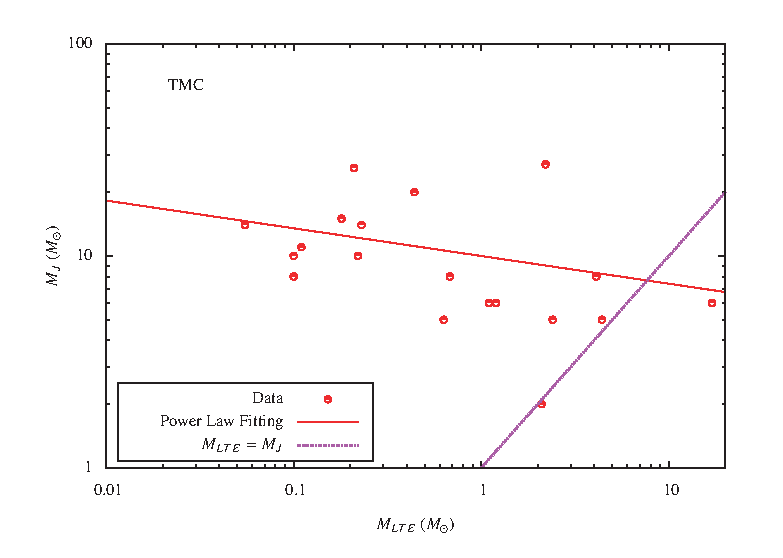
\includegraphics[totalheight=50mm]{img_plot/M_j_tmc.eps}
			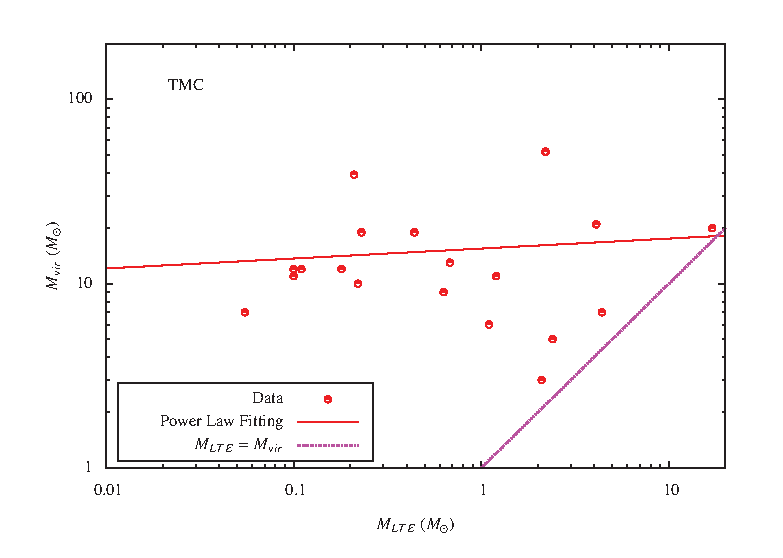
\includegraphics[totalheight=50mm]{img_plot/M_vir_tmc.eps}\\
			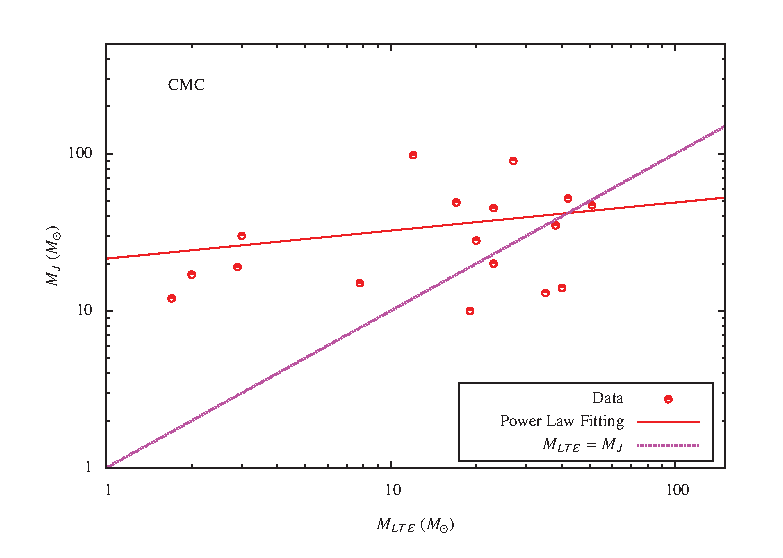
\includegraphics[totalheight=50mm]{img_plot/M_j_cmc.eps}
			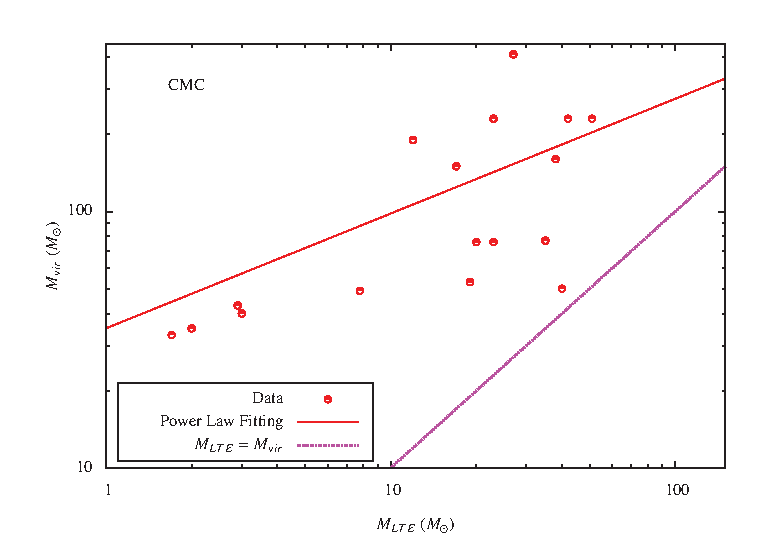
\includegraphics[totalheight=50mm]{img_plot/M_vir_cmc.eps}
			\caption{左上图: TMC中云核的 $M_{LTE}-M_{J}$ 关系;右上图:TMC中云核的 $M_{LTE}-M_{vir}$ 关系;左下图: CMC中云核的 $M_{LTE}-M_{J}$ 关系;右下图:CMC中云核的 $M_{LTE}-M_{vir}$ 关系.  蓝色虚线表示 $M_{LTE}=M_{J}$ 或 $M_{LTE}=M_{vir}$。\label{Fig.Mass}}
		\end{figure}

		通过比较,我们发现TMC的\numcoretmc 个云核中有17个$M_J$大于$M_{LTE}$,这表明他们很可能没有重力作用下的塌缩;对于CMC的\numcorecmc 个云核中有10个$M_J$大于$M_{LTE}$,在其余6个$M_{LTE}>M_J$的云核中,三个(G156.92-09.72C1, G157.12-11.56C1, G157.60-12.17bC1) 被发现有蓝色轮廓的谱线,这表明了其中可能存在重力塌缩。值得注意的是,G157.60-12.17bC1是CMC中唯一一个有\sigmath $>$ \sigmant 的云核,这增加了其存在重力塌缩的可能性。

		与此同时,所有的云核都有$M_{vir}>M_{LTE}$。在TMC中,云核的平均 $\alpha=\frac{M_{vir}}{M_{LTE}}$高达51;在CMC中,这个比值更达到58。在TMC中仅4个云核有$\alpha<3$,而其中的63\%都有$\alpha>10$;对于CMC,$\alpha$的均值为$9\pm6$,仅3个云核有$\alpha<3$。两个区域如此巨大的$\alpha$揭示了他们并未处于重力束缚下,很可能正处在演化的过渡阶段。

		需要强调的是,我们不能忽略分辨率对以上分析准确性的影响。在CMC的距离(450 pc)上,我们采用的望远镜的波束投影直径为$\sim 0.1$ pc,意味着其不能很好分辨典型尺寸($0.03~0.2$ pc)\supercite{2007ARA&A..45..339B}的云核。而考虑到$M_{J}\propto R^{1/2}$、$M_{vir}\propto R$但是 $M_{LTE}\propto R^2$ :我们可能高估了CMC中云核的$M_{LTE}$(相对于$M_{LTE}$和$M_{J}$)。

	\section{气体-尘埃耦合}

		我们研究了全部云核的气体-尘埃热耦合状况。

		由于我们采用了LTE假设,\texc 可以表征云核中气体成分的热运动温度($T_k$)。而云核中尘埃成分的温度可以由Planck的连续谱观测导出。我们直接使用ECC源表中的“TEMPERATURE\_CORE” 一列\supercite{2011yCat.8088....0P},记之为$T_D$。

		对于这些云核的$T_k$ 和 $T_D$之间的比较如图 \ref{Fig.GasDust}所示:
		
		\begin{figure}[htbp]
		\begin{center}
			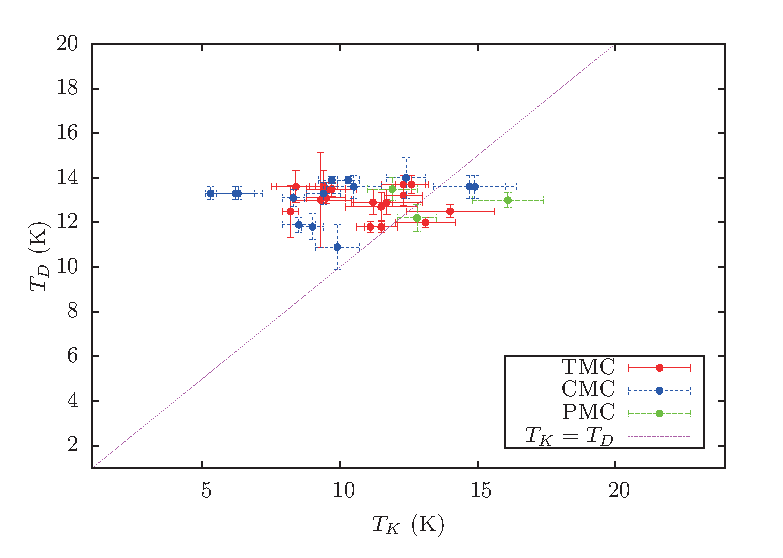
\includegraphics[totalheight=62mm]{img_plot/Gas-Dust_EB_Core.eps}
			\caption{$T_D-T_K$ 关系, $T_K$ 即为各云核的 \texc 而 $T_D$ 为ECC源表\supercite{2011yCat.8088....0P} 中的“TEMPERATURE\_CORE” 一列.\label{Fig.GasDust}}
		\end{center}
		\end{figure}
		
		我们没有发现$T_K$ 和 $T_D$ 之间有任何明显的相关性:例如其线性相关的$R^2\sim 10^{-5}$。 然而,我们发现大部分(61\%)的云核有$T_D>T_K$。对于全部\numcore 个云核,$T_D/T_k$ 的平均值为 1.3$\pm$0.4;对于TMC中的云核,此均值为$1.23\pm0.23$;而对于CMC中的云核,此均值为$1.47\pm0.47$。

		相较于气体温度,大部分云核具有更高的尘埃温度,这可以用“尘埃加热气体”的模型解释:尘埃颗粒被分子云中心恒星形成过程中的辐射所加热,之后通过碰撞将能量传递给比尘埃颗粒冷的气体分子\supercite{1974ApJ...189..441G}。另外,关于耗空(depletion)的物理模型\supercite{2001ApJ...557..736G}显示\nnhyd $<10^{4}\rm\ cm^{-3}$时会有$T_K$的升高, 从而使得$T_D>T_K$。我们样品中云核的\nnhyd 全部在这个范围内(TMC和CMC中云核均有\nnhyd $<10^{3.9}\rm\ cm^{-3}$),但并无$T_D>T_K$,故而不符合此模型。此矛盾很可能揭示了我们的云核尚无显著的耗空,这同样可能是由于我们云核处于早期演化阶段导致的。

		\iffalse
     
     	The comparison of $T_k$ and $T_D$ is as shown in Figure \ref{Fig.GasDust}.
     	The correlation between $T_K$ and $T_D$ is not obvious: which is with $R^2\sim 10^{-5}$. However, we  found that majority (61\%) of the cores have $T_D>T_K$. All the \numcore cores are with the $T_D/T_k$ of  average value 1.3$\pm$0.4. The cores in TMC are with mean $T_D/T_k=1.23\pm0.23$, while the cores in CMC  are with mean $T_D/T_k=1.47\pm0.47$.
 
     	Such excess of dust temperature can be interpreted with the mechanism of gas heated by dust: dust grains  are heated by radiations from forming stellar objects in the center of the molecular clouds, and  transfer energy to cooler gas by collisions (\citealt{1974ApJ...189..441G}). Model of depletion suggests  a increasing of $T_K$ and $T_D<T_K$ when \nnhyd$<10^{4}\rm\ cm^{-3}$ (\citealt{2001ApJ...557..736G}). As  the \nnhyd in TMC and CMC are both less than $10^{3.9}\rm\ cm^{-3}$, our result cannot consist this model . This inconsistency indicates that the depletion in our cores are not significant yet.
\fi
	\section{CO丰度}
	\section{云核的成协情况}

\appendix 

\printbibliography[heading = bibintoc]

\chapter{云核中心光谱}\label{App.Spectra}
	本附录出示云核中心的光谱,如图\ref{Fig.Spectra}.

	\begin{figure}[h]
		\caption{云核中心的光谱.对于每个光谱图,\coaa 、 \cobb 和 \cocc   的谱线分别以红、绿、蓝表示.光谱选取的位置(相对于Planck冷团块几何中心的偏移)标示在云核名称的下方,形式为“(RA,DEC)”, 单位为角分.\label{Fig.Spectra}}
	\end{figure}
		\vspace{-18mm}
		%\begin{center}
\insertspec{G153.34-08.00C1_spec}
\insertspec{G153.34-08.00C2_spec}
\insertspec{G154.68-15.34C1_spec}
\insertspec{G155.52-08.93_spec}
\insertspec{G156.53-08.63_spec}
\insertspec{G156.90-08.49_spec}
\insertspec{G156.92-09.72C1_spec}
\insertspec{G157.10-08.70_spec}
\insertspec{G157.12-11.56C1_spec}
\insertspec{G157.12-11.56C2_spec}
\insertspec{G157.12-11.56C3_spec}
\insertspec{G157.19-08.81_spec}
\insertspec{G157.58-08.89_spec}
\insertspec{G157.60-12.17a_spec}
\insertspec{G157.60-12.17bC1_spec}
\insertspec{G157.60-12.17bC2_spec}
\insertspec{G157.91-08.23C1_spec}
\insertspec{G158.20-20.28_spec}
\insertspec{G158.22-20.14_spec}
\insertspec{G158.24-21.80_spec}
\insertspec{G158.37-20.72_spec}
\insertspec{G158.40-21.86_spec}
\insertspec{G159.01-08.46_spec}
\insertspec{G159.03-08.32_spec}
\insertspec{G159.14-08.76_spec}
\insertspec{G159.16-05.58_spec}
\insertspec{G159.21-20.12C1_spec}
\insertspec{G159.65-19.68a_spec}
\insertspec{G159.65-19.68b_spec}
\insertspec{G159.67-05.71aC1_spec}
\insertspec{G159.67-05.71aC2_spec}
\insertspec{G159.67-05.71bC1_spec}
\insertspec{G159.82-10.48C1_spec}
\insertspec{G159.82-10.48C2_spec}
\insertspec{G160.35-06.37_spec}
\insertspec{G160.51-16.84_spec}
\insertspec{G160.51-17.07_spec}
\insertspec{G160.53-09.84_spec}
\insertspec{G160.53-19.72C1_spec}
\insertspec{G160.62-16.70_spec}
\insertspec{G161.08-21.78_spec}
\insertspec{G161.21-08.72_spec}
\insertspec{G162.24-09.04C1_spec}
\insertspec{G162.46-08.70_spec}
\insertspec{G162.86-05.24_spec}
\insertspec{G163.32-08.42_spec}
\insertspec{G164.13-08.85C1_spec}
\insertspec{G164.57-24.48C1_spec}
\insertspec{G164.57-24.48C2_spec}
\insertspec{G164.57-24.48C3_spec}
\insertspec{G164.75-24.19C1_spec}
\insertspec{G164.75-24.19C2_spec}
\insertspec{G164.81-05.67C1_spec}
\insertspec{G164.92-12.65C1_spec}
\insertspec{G164.92-12.65C2_spec}
\insertspec{G164.92-12.65C3_spec}
\insertspec{G166.99-15.34C1_spec}
\insertspec{G168.00-15.69_spec}
\insertspec{G168.13-16.39a_spec}
\insertspec{G168.13-16.39b_spec}
\insertspec{G169.76-16.15a_spec}
\insertspec{G169.76-16.15b_spec}
\insertspec{G169.82-19.39_spec}
\insertspec{G169.98-18.97_spec}
\insertspec{G170.13-16.06a_spec}
\insertspec{G170.13-16.06b_spec}
\insertspec{G170.26-16.02_spec}
\insertspec{G170.57-07.85_spec}
\insertspec{G170.88-10.92_spec}
\insertspec{G171.43-17.36_spec}
\insertspec{G172.13-16.93_spec}
\insertspec{G172.83-05.17C1_spec}
\insertspec{G172.85-14.74_spec}
\insertspec{G172.92-16.74a_spec}
\insertspec{G172.92-16.74b_spec}
\insertspec{G172.94-05.49C1_spec}
\insertspec{G173.07-17.89C1_spec}
\insertspec{G173.07-17.89C2_spec}
\insertspec{G173.45-05.43_spec}
\insertspec{G173.60-17.89C1_spec}
\insertspec{G173.60-17.89C2_spec}
\insertspec{G173.91-16.25_spec}
\insertspec{G174.06-15.81_spec}
\insertspec{G174.39-13.43_spec}
\insertspec{G174.70-15.48C1_spec}
\insertspec{G175.16-16.74_spec}
\insertspec{G175.97-20.38C1_spec}
\insertspec{G176.46-21.10_spec}
\insertspec{G177.60-20.58_spec}
\insertspec{G177.89-20.16a_spec}
\insertspec{G177.89-20.16b_spec}
\insertspec{G177.97-09.72_spec}
\end{center}

\chapter{各团块积分强度图}\label{App.Map}
	
	本附录出示每个团块的积分强度图,如图\ref{Fig.Map}.

	\begin{figure}[h]
		\caption{等值线图表示\cobb 谱线的积分强度,灰度背景表示\coaa 谱线的积分强度.等值线表示的积分强度范围:由峰值强度的30\% 到 90\%;相邻等值线表示的积分强度差:峰值强度的10\%.图上的蓝色或黄色符号表示成协物:$\times$(X-ray object)、 $\triangle$(radio, {HI}, Maser)、$\Diamond$(IR object)、HH(Herbig-Haro object)、YSO(Young Stellar Object).成协物的种类、位置以及代表符号均根据SIMBAD数据库中的Aladin应用程序.\label{Fig.Map}}
	\end{figure}
		\vspace{-18mm}
		%\begin{center}
\insertmap{G153.34-08.00}
\insertmap{G154.68-15.34}
\insertmap{G155.52-08.93}
\insertmap{G156.53-08.63}
\insertmap{G156.90-08.49}
\insertmap{G156.92-09.72}
\insertmap{G157.10-08.70}
\insertmap{G157.12-11.56}
\insertmap{G157.19-08.81}
\insertmap{G157.58-08.89}
\insertmap{G157.60-12.17}
\insertmap{G157.60-12.17b}
\insertmap{G157.91-08.23}
\insertmap{G158.20-20.28}
\insertmap{G158.22-20.14}
\insertmap{G158.24-21.80}
\insertmap{G158.37-20.72}
\insertmap{G158.40-21.86}
\insertmap{G159.01-08.46}
\insertmap{G159.03-08.32}
\insertmap{G159.14-08.76}
\insertmap{G159.16-05.58}
\insertmap{G159.21-20.12}
\insertmap{G159.65-19.68}
\insertmap{G159.65-19.68b}
\insertmap{G159.67-05.71}
\insertmap{G159.82-10.48}
\insertmap{G160.35-06.37}
\insertmap{G160.51-16.84}
\insertmap{G160.51-17.07}
\insertmap{G160.53-09.84}
\insertmap{G160.53-19.72}
\insertmap{G160.62-16.70}
\insertmap{G161.08-21.78}
\insertmap{G161.21-08.72}
\insertmap{G162.24-09.04}
\insertmap{G162.46-08.70}
\insertmap{G162.86-05.24}
\insertmap{G163.32-08.42}
\insertmap{G164.13-08.85}
\insertmap{G164.57-24.48}
\insertmap{G164.75-24.19}
\insertmap{G164.81-05.67}
\insertmap{G164.92-12.65}
\insertmap{G166.99-15.34}
\insertmap{G168.00-15.69}
\insertmap{G168.13-16.39}
\insertmap{G169.76-16.15}
\insertmap{G169.76-16.15b}
\insertmap{G169.82-19.39}
\insertmap{G169.98-18.97}
\insertmap{G170.13-16.06}
\insertmap{G170.26-16.02}
\insertmap{G170.57-07.85}
\insertmap{G170.88-10.92}
\insertmap{G171.43-17.36}
\insertmap{G172.13-16.93}
\insertmap{G172.83-05.17}
\insertmap{G172.85-14.74}
\insertmap{G172.92-16.74}
\insertmap{G172.92-16.74b}
\insertmap{G172.94-05.49}
\insertmap{G173.07-17.89}
\insertmap{G173.45-05.43}
\insertmap{G173.60-17.89}
\insertmap{G173.91-16.25}
\insertmap{G174.06-15.81}
\insertmap{G174.39-13.43}
\insertmap{G174.70-15.48}
\insertmap{G175.16-16.74}
\insertmap{G175.97-20.38}
\insertmap{G176.46-21.10}
\insertmap{G177.60-20.58}
\insertmap{G177.89-20.16}
\insertmap{G177.89-20.16b}
\insertmap{G177.97-09.72}
\insertmap{void}
\insertmap{void}
\end{center}	

\backmatter

% vim:ts=4:sw=4
%
% Copyright (c) 2008-2009 solvethis
% Copyright (c) 2010-2012 Casper Ti. Vector
% Public domain.

\chapter{致谢}

首先,由衷地感谢我的导师,北京大学天文学系吴月芳教授。我大学二年级伊始,她的谆谆教诲和辛勤辅导引导我开始了天体物理学的研究。近三年来,吴教授一方面细致耐心地指导我的学习和科研,同时也亲切地关心我生活的各个方面。在我本科期间,吴老师支持并资助我三次赴中国科学院紫金山天文台青海观测站进行观测实习,并且鼓励我参与“\emph{Planck}冷团块的气体成分观测”这样意义重大的课题,同时耐心指导我独立完成本文展示的这部分研究。吴教授不仅传授给我天体物理学的思想、知识和方法,她严谨的治学态度和实事求是、追求卓越的科学精神亦将使我终生受用。

感谢同一课题组刘铁的指导和帮助。2011年1月,他在青海观测站辅导我掌握了基本的观测和数据处理方法。之后又不断就研究中的问题给予我耐心的指导。本文中的数据处理用的程序正是基于他编写的脚本而修改得到的。

感谢中国科学院紫金山天文台青海观测站的巨炳刚、孙继先和逯登荣等老师、工程师和全体工作人员。他们的辛勤工作和耐心指导使得我们的观测得以顺利进行,同时他们的细致讲解使得我对射电天文观测有了基本的了解。

感谢天文学系和KIAA的各位老师,他们所讲授的课程和组织的报告与讨论使我有了从事本研究的知识基础和技能储备。特别是:徐仁新老师讲授的《天体物理》,刘富坤老师与刘晓为老师讲授的《恒星大气与天体光谱》,黄茂海老师、卢方军老师和张华伟老师讲授的《天文技术与方法》以及天文学习2907教室丰富多彩的“午餐报告”和KIAA举办的“本科生学术讨论会”,这些课程和讨论会让我获得了知识和技能,也使我由衷地感受到天文学带来的快乐。

感谢同一课题组的任致远、王科、孙宁晨、刘博洋、王文慧、龙凤以及罗连通。他们对我的帮助和与我进行的讨论使我受益匪浅。

篇幅所限,在此对其余所有对本研究作出了贡献的个人和组织表示感谢。


% vim:ts=4:sw=4
%
% Copyright (c) 2008-2009 solvethis
% Copyright (c) 2010-2012 Casper Ti. Vector
% All rights reserved.
%
% Redistribution and use in source and binary forms, with or without
% modification, are permitted provided that the following conditions are
% met:
%
% * Redistributions of source code must retain the above copyright notice,
%   this list of conditions and the following disclaimer.
% * Redistributions in binary form must reproduce the above copyright
%   notice, this list of conditions and the following disclaimer in the
%   documentation and/or other materials provided with the distribution.
% * Neither the name of Peking University nor the names of its contributors
%   may be used to endorse or promote products derived from this software
%   without specific prior written permission.
% 
% THIS SOFTWARE IS PROVIDED BY THE COPYRIGHT HOLDERS AND CONTRIBUTORS "AS
% IS" AND ANY EXPRESS OR IMPLIED WARRANTIES, INCLUDING, BUT NOT LIMITED TO,
% THE IMPLIED WARRANTIES OF MERCHANTABILITY AND FITNESS FOR A PARTICULAR
% PURPOSE ARE DISCLAIMED. IN NO EVENT SHALL THE COPYRIGHT HOLDER OR
% CONTRIBUTORS BE LIABLE FOR ANY DIRECT, INDIRECT, INCIDENTAL, SPECIAL,
% EXEMPLARY, OR CONSEQUENTIAL DAMAGES (INCLUDING, BUT NOT LIMITED TO,
% PROCUREMENT OF SUBSTITUTE GOODS OR SERVICES; LOSS OF USE, DATA, OR
% PROFITS; OR BUSINESS INTERRUPTION) HOWEVER CAUSED AND ON ANY THEORY OF
% LIABILITY, WHETHER IN CONTRACT, STRICT LIABILITY, OR TORT (INCLUDING
% NEGLIGENCE OR OTHERWISE) ARISING IN ANY WAY OUT OF THE USE OF THIS
% SOFTWARE, EVEN IF ADVISED OF THE POSSIBILITY OF SUCH DAMAGE.

% 原创性声明和使用授权说明页不需要装订到论文中,故不显示页码。
\cleardoublepage\thispagestyle{empty}
{
	\linespread{1.5}\selectfont
	\section*{北京大学学位论文原创性声明和使用授权说明}

	\vfill
	\section*{原创性声明}

	本人郑重声明:
	所呈交的学位论文,是本人在导师的指导下,独立进行研究工作所取得的成果。
	除文中已经注明引用的内容外,
	本论文不含任何其他个人或集体已经发表或撰写过的作品或成果。
	对本文的研究做出重要贡献的个人和集体,均已在文中以明确方式标明。
	本声明的法律结果由本人承担。
	\vspace{2.5em}\par
	\rightline
	{%
		论文作者签名:\hspace{5em}%
		日期:\hspace{2em}年\hspace{2em}月\hspace{2em}日%
	}

	\vfill
	\section*{学位论文使用授权说明}
	\vspace{-1em}\par
	\centerline{\zihao{-4}(必须装订在提交学校图书馆的印刷本)}
	\vspace{1em}\par

	本人完全了解北京大学关于收集、保存、使用学位论文的规定,即:
	\begin{itemize}
		\item 按照学校要求提交学位论文的印刷本和电子版本;
		\item 学校有权保存学位论文的印刷本和电子版,
			并提供目录检索与阅览服务,在校园网上提供服务;
		\item 学校可以采用影印、缩印、数字化或其它复制手段保存论文;
		\item 因某种特殊原因需要延迟发布学位论文电子版,
			授权学校在 $\square$\nobreakspace{}一年 / %
			$\square$\nobreakspace{}两年 / %
			$\square$\nobreakspace{}三年以后在校园网上全文发布。
	\end{itemize}
	\par(保密论文在解密后遵守此规定)
	\vspace{2.5em}\par
	\rightline
	{%
		论文作者签名:\hspace{5em}导师签名:\hspace{5em}%
		日期:\hspace{2em}年\hspace{2em}月\hspace{2em}日%
	}
	\par
}


\end{document}

